\section{Geometry configuration}
\label{sec:GeoConf}

In this section are described the different elements for a geometry configuration as well as 
the syntax for the specification of the world volume, magnetic field, different geometry elements, 
resolution model, efficiency model, and systems and Telescope-DUT configurations.

In {\guari} there is an internal unit system. All physical quantities have to be specified with the corresponding units, 
otherwise the program will crash with an error message.

The volumes in space are placed by specifying a position and a set of three rotation angles $(\alpha_x,\alpha_y,\alpha_z)$ to 
determine its orientation. The rotation convention is 

\begin{equation}
  R = R_z(\alpha_x) R_z(\alpha_y) R_z(\alpha_z) 
\end{equation}
\noindent
where $R$ is the full rotation matrix, and $R_i(\alpha_i)$ are rotation matrices along the axis-$i$ by an angle $\alpha_i$. 
The rotation order if along the z-axis first, then along the y-axis and finally along the x-axis. The specification of the 
rotation angles is not mandatory, if not specified they will all be set to its default value $(0,0,0)$.


\subsection{World volume}

The world volume should contain all the geometry elements, and only inside it the track navigation will 
be performed. Currently, only two kinds of world volumes are possible, either a box or a cylinder. The specification 
is as follows,

\subsubsection{Box world volume}

The box world volume is specified as follows,
~\\
~\\
\noindent
{\tt BeginBoxWorldVolume} \\
$~~~~~${\tt Position   x   y   z  units   // (Mandatory)} \\
$~~~~~${\tt widthX     value  units  $~$  // (Mandatory, value > 0)} \\
$~~~~~${\tt widthY     value  units  $~$  // (Mandatory, value > 0)} \\
$~~~~~${\tt widthZ     value  units  $~$  // (Mandatory, value > 0)} \\
{\tt EndBoxWorldVolume} \\

\noindent
where {\tt Position} specifies the center of the box, and {\tt widthX,Y,Z} the widths along the global frame axes.

\subsubsection{Cylinder world volume}

The cylinder world volume is specified as follows,

\noindent
{\tt BeginCylinderWorldVolume} \\
$~~~~~${\tt Position   x   y   z  units  // (Mandatory)} \\
$~~~~~${\tt Radius     value  units  $~$ // (Mandatory, value > 0)} \\
$~~~~~${\tt Length     value  units  $~$ // (Mandatory, value > 0)} \\
{\tt EndCylinderWorldVolume} \\

\noindent
where {\tt Position} specifies the center of the cylinder. The other parameters are evident. The cylinder is always oriented along the 
global z-axis.

\subsection{Magnetic field}

Each geometry has its own magnetic field. If not specified it is assumed to be zero. Two types of B-field 
are currently implemented.

\subsubsection{Constant Magnetic field}

A constant B-field is build by specifying its magnitude and direction as shown below.
~\\
~\\
\noindent
{\tt BeginConstantBfield} \\
$~~~~~${\tt Magnitude    value  units      // (Mandatory, value > 0)} \\
$~~~~~${\tt Direction    x  y  z   $~~~~~$ // (Mandatory, vector will be normalized to unity)} \\
{\tt EndConstantBfield}

\subsubsection{Piece-wise Magnetic field}

This magnetic field consist of a set of non-overlapping volumes with a constant B-field inside each of them. If any pair of the 
specified volumes overlap, the program will crash with an error message. Outside all the volumes the B-field is zero by default, 
but it can be set to a non-zero values if specified. A set of volumes of different types can be specified. A set of so-called 
"inside-fields" have to be specified as well. The number of volumes have to match the number of inside-fields, otherwise the 
program will crash with an error message. The syntax for specifying this kind of B-field is as follows.

~\\
~\\
\noindent
{\tt BeginMultipleStepsBfield} \\
$~~~~~${\tt BeginSomeTypeVolume} \\
$~~~~~~~${...} \\
$~~~~~${\tt EndSomeTypeVolume}   \\
$~~~~~${\tt BeginInsideBfield} \\
$~~~~~~~${\tt Magnitude    value  units      // (Mandatory, value > 0)} \\
$~~~~~~~${\tt Direction    x  y  z   $~~~~~$ // (Mandatory, vector will be normalized to unity)} \\
$~~~~~${\tt EndInsideBfield} \\
$~~~~~${\tt ...} \\
$~~~~~${\tt BeginOutsideBfield} \\
$~~~~~~~${\tt Magnitude    value  units      // (Mandatory, value > 0)} \\
$~~~~~~~${\tt Direction    x  y  z   $~~~~~$ // (Mandatory, vector will be normalized to unity)} \\
$~~~~~${\tt EndOutsideBfield} \\
{\tt EndMultipleStepsBfield}

~\\
\noindent
The data structure inside {\tt BeginOutsideBfield} and {\tt EndOutsideBfield} is optional. If not specified 
then the "outside-field" will be set to zero. 

The {\tt SomeType} on {\tt BeginSomeTypeVolume} and {\tt EndSomeTypeVolume} represents the different types of 
volumes which can be specified, each of them with their own syntax. There are several volume types which are mentioned 
here below.

\begin{itemize}
  \item  {\bf Box volume}: specified as follows,

  \noindent
  {\tt BeginBoxVolume} \\
  $~~~~~${\tt Position   x  y  z  units                       $~~~$ // (Mandatory)} \\
  $~~~~~${\tt RotAngles  $\alpha_x$  $\alpha_x$  $\alpha_x$  units  // (Optional)} \\
  $~~~~~${\tt widthX     value   units                      $~~~~~$ // (Mandatory, value > 0)} \\
  $~~~~~${\tt widthY     value   units                      $~~~~~$ // (Mandatory, value > 0)} \\
  $~~~~~${\tt widthZ     value   units                      $~~~~~$ // (Mandatory, value > 0)} \\
  {\tt EndBoxVolume}
  
  \item {\bf Cylinder volume}: specified as follows,
  
  \noindent
  {\tt BeginCylinderVolume} \\
  $~~~~~${\tt Position   x  y  z  units                       $~~~$ // (Mandatory)} \\
  $~~~~~${\tt RotAngles  $\alpha_x$  $\alpha_x$  $\alpha_x$  units  // (Optional)} \\
  $~~~~~${\tt Radius     value   units                      $~~~~~$ // (Mandatory, value > 0)} \\
  $~~~~~${\tt Length     value   units                      $~~~~~$ // (Mandatory, value > 0)} \\
  {\tt EndCylinderVolume}
  
  \item {\bf Cone volume}: specified as follows,
  
  \noindent
  {\tt BeginConeVolume} \\
  $~~~~~${\tt Position   x  y  z  units                       $~~~$ // (Mandatory)} \\
  $~~~~~${\tt RotAngles  $\alpha_x$  $\alpha_x$  $\alpha_x$  units  // (Optional)} \\
  $~~~~~${\tt Radius1    value   units                       $~~~~$ // (Mandatory, value > 0)} \\
  $~~~~~${\tt Radius2    value   units                       $~~~~$ // (Mandatory, value > 0)} \\
  $~~~~~${\tt Length     value   units                      $~~~~~$ // (Mandatory, value > 0)} \\
  {\tt EndConeVolume}
  
  \item {\bf Disk section volume}: specified as follows,
  
  \noindent
  {\tt BeginDiskSectionVolume} \\
  $~~~~~${\tt Position   x  y  z  units                       $~~~$ // (Mandatory)} \\
  $~~~~~${\tt RotAngles  $\alpha_x$  $\alpha_x$  $\alpha_x$  units  // (Optional)} \\
  $~~~~~${\tt Rin        value   units                   $~~~~~~~~$ // (Mandatory, value > 0)} \\
  $~~~~~${\tt Rout       value   units                    $~~~~~~~$ // (Mandatory, value > 0)} \\
  $~~~~~${\tt Length     value   units                      $~~~~~$ // (Mandatory, value > 0)} \\
  $~~~~~${\tt DeltaPhi   value   units                        $~~~$ // (Mandatory, value > 0)} \\
  {\tt EndDiskSectionVolume}
  
  \noindent
  The disk section will expand an angle {\tt DeltaPhi} around the local x-axis.
  
  \item {\bf Cone section volume}: specified as follows,
  
  \noindent
  {\tt BeginConeSectionVolume} \\
  $~~~~~${\tt Position   x  y  z  units                       $~~~$ // (Mandatory)} \\
  $~~~~~${\tt RotAngles  $\alpha_x$  $\alpha_x$  $\alpha_x$  units  // (Optional)} \\
  $~~~~~${\tt Radius1    value   units                       $~~~~$ // (Mandatory, value > 0)} \\
  $~~~~~${\tt Radius2    value   units                       $~~~~$ // (Mandatory, value > 0)} \\
  $~~~~~${\tt Length     value   units                      $~~~~~$ // (Mandatory, value > 0)} \\
  $~~~~~${\tt DeltaPhi   value   units                        $~~~$ // (Mandatory, value > 0)} \\
  {\tt EndConeSectionVolume}
  
  \noindent
  The cone section will expand an angle {\tt DeltaPhi} around the local x-axis.
  
\end{itemize}


As an example, here below there is an example of a piece-wise B-field with two cylindric volumes along the z-axis with fields pointing 
in opposite directions, both along the x-axis.

~\\
\noindent
{\tt BeginMultipleStepsBfield} \\
$~~~~~${\tt BeginCylinderVolume} \\
$~~~~~~~${\tt Position   0.0 0.0 0.0 cm} \\
$~~~~~~~${\tt RotAngles  0.0 0.0 0.0 deg} \\
$~~~~~~~${\tt Radius     5.0  cm} \\
$~~~~~~~${\tt Length     2.0  cm} \\
$~~~~~${\tt EndCylinderVolume} \\
$~~~~~${\tt BeginInsideBfield} \\
$~~~~~~~${\tt Magnitude    1.0 T} \\
$~~~~~~~${\tt Direction    1 0 0} \\
$~~~~~${\tt EndInsideBfield} \\
$~~~~~${\tt BeginCylinderVolume} \\
$~~~~~~~${\tt Position   0.0 0.0 10.0 cm} \\
$~~~~~~~${\tt RotAngles  0.0 0.0  0.0 deg} \\
$~~~~~~~${\tt Radius     5.0  cm} \\
$~~~~~~~${\tt Length     2.0  cm} \\
$~~~~~${\tt EndCylinderVolume} \\
$~~~~~${\tt BeginInsideBfield} \\
$~~~~~~~${\tt Magnitude    1.0 T} \\
$~~~~~~~${\tt Direction   -1 0 0} \\
$~~~~~${\tt EndInsideBfield} \\
$~~~~~${\tt BeginOutsideBfield} \\
$~~~~~~~${\tt Magnitude    0.5 T} \\
$~~~~~~~${\tt Direction    0 1 0} \\
$~~~~~${\tt EndOutsideBfield} \\
{\tt EndMultipleStepsBfield}

\subsection{Simple geometries}

In this section will be described the syntax for the geometrical volumes up to now implemented in {\guari}. 
A complex geometry will be build using the simple geometrical volumes described in the sections below. In the 
specification of a geometry element a set of parameters are always mandatory, those which allow to place the 
volume on space and to assign its material properties. These volumes could be sensitive, {\it i.e.} detector, 
depending on the value of the bool variable {\tt IsSensitive}. In case it is set to {\tt true}, then the specification 
of additional parameters becomes mandatory. Those parameters refers to the detection performances of the sensitive 
element, such as intrinsic resolution ({\tt ResolutionU/V}), detection efficiency ({\tt Efficiency}), readout time 
({\tt ROtime}) and insensitive borders ({\tt InsensFracU/Vneg} and {\tt InsensFracU/Vpos}). The amount of hit rate 
({\tt BkgRate}, hits per unit of time and unit of surface) can also be specified. It is mainly used in the calculation 
of the tracking efficiency.

~\\
Lets now describe the syntax of the different geometrical volumes. The meaning of some parameters common to all
volumes will be fully described in the section~\ref{subsubsec:Plane}.

\subsubsection{Plane}
\label{subsubsec:Plane}

A so-called {\tt GeoPlane}, is a box in which one of its dimensions is much smaller than the other two. Its 
syntax is as follows,

~\\
\noindent
{\tt BeginGeoPlane} \\
$~~~~~${\tt Name             string                   $~~~~~~~~~~~~$   // (Mandatory)} \\
$~~~~~${\tt Position         x  y  z units                     $~~~$   // (Mandatory)} \\
$~~~~~${\tt RotAngles        $\alpha_x$  $\alpha_y$  $\alpha_z$ units  // (Optional)}  \\
$~~~~~${\tt Thickness        value  units                       $~~$   // (Mandatory, value > 0)} \\
$~~~~~${\tt Material         string                       $~~~~~~~~$   // (Mandatory)} \\
$~~~~~${\tt XOX0             value                   $~~~~~~~~~~~~~$   // (Optional)}  \\
$~~~~~${\tt widthU           value units                     $~~~~~$   // (Mandatory, value > 0)} \\
$~~~~~${\tt widthV           value units                     $~~~~~$   // (Mandatory, value > 0)} \\
$~~~~~${\tt IsSensitive      bool                          $~~~~~~~$   // (Mandatory)} \\
$~~~~~${\tt ResolutionU      value units                               // (Optional, value > 0)} \\
$~~~~~${\tt ResolutionV      value units                               // (Optional, value > 0)} \\
$~~~~~${\tt Resolution       value units                               // (Optional, value > 0)} \\
$~~~~~${\tt ROtime           value units                      $~~~~$   // (Optional, value > 0)} \\
$~~~~~${\tt Efficiency       value                          $~~~~~~$   // (Optional, 0 <= value <= 1)} \\
$~~~~~${\tt InsensFracUneg   value                              $~~$   // (Optional, default is zero)} \\
$~~~~~${\tt InsensFracUpos   value                              $~~$   // (Optional, default is zero)} \\
$~~~~~${\tt InsensFracVneg   value                              $~~$   // (Optional, default is zero)} \\
$~~~~~${\tt InsensFracVpos   value                              $~~$   // (Optional, default is zero)} \\
$~~~~~${\tt BkgRate          value units                       $~~~$   // (Optional, default is zero)} \\
$~~~~~${\tt SystemName       string                          $~~~~~$   // (Optional)} \\
$~~~~~${\tt LayerName        string                         $~~~~~~$   // (Optional)} \\
$~~~~~${\tt ResolutionModel  string                                    // (Optional)} \\
$~~~~~${\tt EfficiencyModel  string                                    // (Optional)} \\
{\tt EndGeoPlane}

~\\
The material budget in units of radiation lengths seen by a particle traversing some path $x$ the volume is calculated using the {\tt Material} 
name. {\guari} has a table of materials with their corresponding $X_0$. The material budget in then simply $x/X_0$. The material budget of a 
given element at normal incidence can be set by hand with the parameter {\tt XOX0}. If it is set, then the material budget at normal incidence, 
{\it i.e.} for a traversed path equal to the thickness, becomes {\tt XOX0}, and the material budget of an arbitrary path $x$ becomes 
$x/X_0 = (x/{\rm Thickness})\times${\tt XOX0}. This feature is useful when to model the material budget of a complicated composite of 
materials like a ladder with sensors, where several material are used to build the object: sensors, cables, supports, ... With this feature a 
single value of {\tt XOX0} has to be specified. This same feature is shared by all the other geometrical volumes.

The variables $U$ and $V$ above refer to the local coordinates on the so-called "main-surface" of the volume. It is 
a plane in the middle of the volume which is used as reference for the local reference frame. In the case of the 
{\tt GeoPlane} object, the main surface is a plane in the middle of the thickness, located at {\tt Position} with the 
{\tt RotAngles} orientation, and with widths {\tt widthU} and {\tt widthV}.

If the {\tt IsSensitive} parameter is set to {\tt true} the intrinsic resolutions along the local $U$ and $V$ directions 
has to be specified. They can be specified separately with the {\tt ResolutionU} and {\tt ResolutionV} parameters, or if 
they are the same it is only needed to specify the {\tt Resolution} parameter ({\tt ResolutionU/V = Resolution}).

The {\tt InsensFracUneg} and {\tt InsensFracUpos} only count for the case of {\tt IsSensitive} set to {\tt true}. These can be used to specify 
an insensitive length at the borders of the {\tt GeoPlane}. These parameters are fractions, {\it i.e.} the values they can have are inside
$[0,1]$, and their sum cannot exceed 1. The insensitive length at the low-edge (high-edge) along the local $U$ coordinate is calculated as 
{\tt InsensFracUneg}$\times${\tt widthU} ({\tt InsensFracUpos}$\times${\tt widthU}). So, even if a particle traverses the volume it can do it 
in a non-sensitive region. In such a case this intersection contributes with no measurement but only with material budget.
The parameters {\tt InsensFraVcneg} and {\tt InsensFracVpos} have a similar meaning.

The {\tt SystemName} and {\tt LayerName} parameters are optional. See the examples in section~\ref{subsec:Some_examples} for 
the usage of these parameters.

The {\tt ResolutionModel} parameter is a string referring to the name of an {\tt GResolutionModel} object. This object calculates 
the sensitive element spatial resolution of the measured point as a function of the intrinsic resolutions ({\tt ResolutionU/V}), 
the intersection coordinates and momentum of the particle with the main surface, and some other parameters. Its default value is an 
empty string, in such case the measurement spatial resolution is equal to the intrinsic resolution. See the example in 
section~\ref{subsubsec:Example3} for an illustration on how it can be used.

Finally, the {\tt EfficiencyModel} parameter is a string referring to the name of an {\tt GEfficiencyModel} object. This object 
calculates the sensitive element detection efficiency of the measured point point as a function of the intrinsic detection efficiency 
({\tt Efficiency}), the intersection coordinates and momentum of the particle with the main surface, and some other parameters. Its default 
value is an empty string, in such case the measurement detection efficiency is equal to the intrinsic detection efficiency.

\subsubsection{Cylinder}
\label{subsubsec:Cylinder}

A so-called {\tt GeoCylinder}, is a cylinder with a small radial thickness. Its syntax is as follows,

~\\
\noindent
{\tt BeginGeoCylinder} \\
$~~~~~${\tt Name             string                   $~~~~~~~~~~~~$   // (Mandatory)} \\
$~~~~~${\tt Position         x  y  z units                     $~~~$   // (Mandatory)} \\
$~~~~~${\tt RotAngles        $\alpha_x$  $\alpha_y$  $\alpha_z$ units  // (Optional)}  \\
$~~~~~${\tt Thickness        value  units                       $~~$   // (Mandatory, value > 0)} \\
$~~~~~${\tt Material         string                       $~~~~~~~~$   // (Mandatory)} \\
$~~~~~${\tt XOX0             value                   $~~~~~~~~~~~~~$   // (Optional)}  \\
$~~~~~${\tt Radius           value units                     $~~~~~$   // (Mandatory, value > 0)} \\
$~~~~~${\tt Length           value units                     $~~~~~$   // (Mandatory, value > 0)} \\
$~~~~~${\tt IsSensitive      bool                          $~~~~~~~$   // (Mandatory)} \\
$~~~~~${\tt ResolutionU      value units                               // (Optional, value > 0)} \\
$~~~~~${\tt ResolutionV      value units                               // (Optional, value > 0)} \\
$~~~~~${\tt Resolution       value units                               // (Optional, value > 0)} \\
$~~~~~${\tt ROtime           value units                      $~~~~$   // (Optional, value > 0)} \\
$~~~~~${\tt Efficiency       value                          $~~~~~~$   // (Optional, 0 <= value <= 1)} \\
$~~~~~${\tt InsensFracVneg   value                              $~~$   // (Optional, default is zero)} \\
$~~~~~${\tt InsensFracVpos   value                              $~~$   // (Optional, default is zero)} \\
$~~~~~${\tt BkgRate          value units                       $~~~$   // (Optional, default is zero)} \\
$~~~~~${\tt SystemName       string                          $~~~~~$   // (Optional)} \\
$~~~~~${\tt LayerName        string                         $~~~~~~$   // (Optional)} \\
$~~~~~${\tt ResolutionModel  string                                    // (Optional)} \\
$~~~~~${\tt EfficiencyModel  string                                    // (Optional)} \\
{\tt EndGeoCylinder}

~\\
In the case of the {\tt GeoCylinder} object, the main surface is a cylinder in the middle of the thickness, located 
at {\tt Position} with the {\tt RotAngles} orientation, and {\tt Radius} and {\tt Length}. The $V$ coordinate goes 
along the cylinder axis, while the $U$ coordinate goes around the circle for fixed $V$.

For a full discussion of all the other parameters see section~\ref{subsubsec:Plane}.


\subsubsection{Cylinder Section}

A so-called {\tt GeoCylinderSection}, is a section of a cylinder with a small radial thickness. Its syntax is as follows,

~\\
\noindent
{\tt BeginGeoCylinderSection} \\
$~~~~~${\tt Name             string                   $~~~~~~~~~~~~$   // (Mandatory)} \\
$~~~~~${\tt Position         x  y  z units                     $~~~$   // (Mandatory)} \\
$~~~~~${\tt RotAngles        $\alpha_x$  $\alpha_y$  $\alpha_z$ units  // (Optional)}  \\
$~~~~~${\tt Thickness        value  units                       $~~$   // (Mandatory, value > 0)} \\
$~~~~~${\tt Material         string                       $~~~~~~~~$   // (Mandatory)} \\
$~~~~~${\tt XOX0             value                   $~~~~~~~~~~~~~$   // (Optional)}  \\
$~~~~~${\tt Radius           value units                     $~~~~~$   // (Mandatory, value > 0)} \\
$~~~~~${\tt Length           value units                     $~~~~~$   // (Mandatory, value > 0)} \\
$~~~~~${\tt DeltaPhi         value units                     $~~~~~$   // (Mandatory, value > 0)} \\
$~~~~~${\tt IsSensitive      bool                          $~~~~~~~$   // (Mandatory)} \\
$~~~~~${\tt ResolutionU      value units                               // (Optional, value > 0)} \\
$~~~~~${\tt ResolutionV      value units                               // (Optional, value > 0)} \\
$~~~~~${\tt Resolution       value units                               // (Optional, value > 0)} \\
$~~~~~${\tt ROtime           value units                      $~~~~$   // (Optional, value > 0)} \\
$~~~~~${\tt Efficiency       value                          $~~~~~~$   // (Optional, 0 <= value <= 1)} \\
$~~~~~${\tt InsensFracVneg   value                              $~~$   // (Optional, default is zero)} \\
$~~~~~${\tt InsensFracVpos   value                              $~~$   // (Optional, default is zero)} \\
$~~~~~${\tt BkgRate          value units                       $~~~$   // (Optional, default is zero)} \\
$~~~~~${\tt SystemName       string                          $~~~~~$   // (Optional)} \\
$~~~~~${\tt LayerName        string                         $~~~~~~$   // (Optional)} \\
$~~~~~${\tt ResolutionModel  string                                    // (Optional)} \\
$~~~~~${\tt EfficiencyModel  string                                    // (Optional)} \\
{\tt EndGeoCylinderSection}

~\\
In the case of the {\tt GeoCylinder} object, the main surface is a section of a cylinder in the middle of the thickness, 
located at {\tt Position} with the {\tt RotAngles} orientation, {\tt Radius} and {\tt Length}, and aperture {\tt DeltaPhi}. 
The $V$ coordinate goes along the cylinder axis, while the $U$ coordinate goes around the circle section for fixed $V$.

For a full discussion of all the other parameters see section~\ref{subsubsec:Plane}.

\subsubsection{Disk}

A so-called {\tt GeoDisk}, is a disk with a small thickness. Its syntax is as follows,

~\\
\noindent
{\tt BeginGeoDisk} \\
$~~~~~${\tt Name             string                   $~~~~~~~~~~~~$   // (Mandatory)} \\
$~~~~~${\tt Position         x  y  z units                     $~~~$   // (Mandatory)} \\
$~~~~~${\tt RotAngles        $\alpha_x$  $\alpha_y$  $\alpha_z$ units  // (Optional)}  \\
$~~~~~${\tt Thickness        value  units                       $~~$   // (Mandatory, value > 0)} \\
$~~~~~${\tt Material         string                       $~~~~~~~~$   // (Mandatory)} \\
$~~~~~${\tt XOX0             value                   $~~~~~~~~~~~~~$   // (Optional)}  \\
$~~~~~${\tt Rin              value units                     $~~~~~$   // (Mandatory, value > 0)} \\
$~~~~~${\tt Rout             value units                     $~~~~~$   // (Mandatory, value > 0)} \\
$~~~~~${\tt IsSensitive      bool                          $~~~~~~~$   // (Mandatory)} \\
$~~~~~${\tt ResolutionU      value units                               // (Optional, value > 0)} \\
$~~~~~${\tt ResolutionV      value units                               // (Optional, value > 0)} \\
$~~~~~${\tt Resolution       value units                               // (Optional, value > 0)} \\
$~~~~~${\tt ROtime           value units                      $~~~~$   // (Optional, value > 0)} \\
$~~~~~${\tt Efficiency       value                          $~~~~~~$   // (Optional, 0 <= value <= 1)} \\
$~~~~~${\tt InsensFracVneg   value                              $~~$   // (Optional, default is zero)} \\
$~~~~~${\tt InsensFracVpos   value                              $~~$   // (Optional, default is zero)} \\
$~~~~~${\tt BkgRate          value units                       $~~~$   // (Optional, default is zero)} \\
$~~~~~${\tt SystemName       string                          $~~~~~$   // (Optional)} \\
$~~~~~${\tt LayerName        string                         $~~~~~~$   // (Optional)} \\
$~~~~~${\tt ResolutionModel  string                                    // (Optional)} \\
$~~~~~${\tt EfficiencyModel  string                                    // (Optional)} \\
{\tt EndGeoDisk}

~\\
In the case of the {\tt GeoDisk} object, the main surface is a disk in the middle of the thickness, located at {\tt Position} with the 
{\tt RotAngles} orientation, and inner and outer radii {\tt Rin} and {\tt Rout}, respectively. The $V$ coordinate goes radially, while the 
$U$ coordinate goes around the circle for fixed $V$.

For a full discussion of all the other parameters see section~\ref{subsubsec:Plane}.

\subsubsection{Disk Section}

A so-called {\tt GeoDiskSection}, is a section of a disk with a small thickness. Its syntax is as follows,

~\\
\noindent
{\tt BeginGeoDiskSection} \\
$~~~~~${\tt Name             string                   $~~~~~~~~~~~~$   // (Mandatory)} \\
$~~~~~${\tt Position         x  y  z units                     $~~~$   // (Mandatory)} \\
$~~~~~${\tt RotAngles        $\alpha_x$  $\alpha_y$  $\alpha_z$ units  // (Optional)}  \\
$~~~~~${\tt Thickness        value  units                       $~~$   // (Mandatory, value > 0)} \\
$~~~~~${\tt Material         string                       $~~~~~~~~$   // (Mandatory)} \\
$~~~~~${\tt XOX0             value                   $~~~~~~~~~~~~~$   // (Optional)}  \\
$~~~~~${\tt Rin              value units                     $~~~~~$   // (Mandatory, value > 0)} \\
$~~~~~${\tt Rout             value units                     $~~~~~$   // (Mandatory, value > 0)} \\
$~~~~~${\tt DeltaPhi         value units                     $~~~~~$   // (Mandatory, value > 0)} \\
$~~~~~${\tt IsSensitive      bool                          $~~~~~~~$   // (Mandatory)} \\
$~~~~~${\tt ResolutionU      value units                               // (Optional, value > 0)} \\
$~~~~~${\tt ResolutionV      value units                               // (Optional, value > 0)} \\
$~~~~~${\tt Resolution       value units                               // (Optional, value > 0)} \\
$~~~~~${\tt ROtime           value units                      $~~~~$   // (Optional, value > 0)} \\
$~~~~~${\tt Efficiency       value                          $~~~~~~$   // (Optional, 0 <= value <= 1)} \\
$~~~~~${\tt InsensFracVneg   value                              $~~$   // (Optional, default is zero)} \\
$~~~~~${\tt InsensFracVpos   value                              $~~$   // (Optional, default is zero)} \\
$~~~~~${\tt BkgRate          value units                       $~~~$   // (Optional, default is zero)} \\
$~~~~~${\tt SystemName       string                          $~~~~~$   // (Optional)} \\
$~~~~~${\tt LayerName        string                         $~~~~~~$   // (Optional)} \\
$~~~~~${\tt ResolutionModel  string                                    // (Optional)} \\
$~~~~~${\tt EfficiencyModel  string                                    // (Optional)} \\
{\tt EndGeoDiskSection}

~\\
In the case of the {\tt GeoDiskSection} object, the main surface is a section of a disk in the middle of the thickness, located at {\tt Position} with 
the {\tt RotAngles} orientation, inner and outer radii {\tt Radius} and {\tt Length}, respectively, and aperture {\tt DeltaPhi}. 
The $V$ coordinate goes radially, while the $U$ coordinate goes around the circle section for fixed $V$.

For a full discussion of all the other parameters see section~\ref{subsubsec:Plane}.

\subsubsection{Cone}

A so-called {\tt GeoCone}, is a cone with a small radial thicknesses. Its syntax is as follows,

~\\
\noindent
{\tt BeginGeoCone} \\
$~~~~~${\tt Name             string                   $~~~~~~~~~~~~$   // (Mandatory)} \\
$~~~~~${\tt Position         x  y  z units                     $~~~$   // (Mandatory)} \\
$~~~~~${\tt RotAngles        $\alpha_x$  $\alpha_y$  $\alpha_z$ units  // (Optional)}  \\
$~~~~~${\tt Thickness1       value  units                       $~~$   // (Mandatory, value > 0)} \\
$~~~~~${\tt Thickness2       value  units                       $~~$   // (Optional)} \\
$~~~~~${\tt Material         string                       $~~~~~~~~$   // (Mandatory)} \\
$~~~~~${\tt XOX0             value                   $~~~~~~~~~~~~~$   // (Optional)}  \\
$~~~~~${\tt Radius1          value units                     $~~~~~$   // (Mandatory, value > 0)} \\
$~~~~~${\tt Radius2          value units                     $~~~~~$   // (Mandatory, value > 0)} \\
$~~~~~${\tt Length           value units                     $~~~~~$   // (Mandatory, value > 0)} \\
$~~~~~${\tt IsSensitive      bool                          $~~~~~~~$   // (Mandatory)} \\
$~~~~~${\tt ResolutionU      value units                               // (Optional, value > 0)} \\
$~~~~~${\tt ResolutionV      value units                               // (Optional, value > 0)} \\
$~~~~~${\tt Resolution       value units                               // (Optional, value > 0)} \\
$~~~~~${\tt ROtime           value units                      $~~~~$   // (Optional, value > 0)} \\
$~~~~~${\tt Efficiency       value                          $~~~~~~$   // (Optional, 0 <= value <= 1)} \\
$~~~~~${\tt InsensFracVneg   value                              $~~$   // (Optional, default is zero)} \\
$~~~~~${\tt InsensFracVpos   value                              $~~$   // (Optional, default is zero)} \\
$~~~~~${\tt BkgRate          value units                       $~~~$   // (Optional, default is zero)} \\
$~~~~~${\tt SystemName       string                          $~~~~~$   // (Optional)} \\
$~~~~~${\tt LayerName        string                         $~~~~~~$   // (Optional)} \\
$~~~~~${\tt ResolutionModel  string                                    // (Optional)} \\
$~~~~~${\tt EfficiencyModel  string                                    // (Optional)} \\
{\tt EndGeoCone}

~\\
In the case of the {\tt GeoCone} object, the main surface is a cone in the middle of its thicknesses, located at {\tt Position} with the {\tt RotAngles}
orientation, and radii at the low-edges and high-edges along its axis of {\tt Radius1} and {\tt Radius2}, respectively, and {\tt Length}. The 
{\tt Thickness1} ({\tt Thickness2}) parameter refers to the thickness at the low-edge (high-edge) of the cone. {\tt Thickness2} is optional, if not 
specified then the same thickness will be used for both edges. The $V$ coordinate goes along the cone slope, while the $U$ coordinate goes around the 
circle for fixed $V$.

For a full discussion of all the other parameters see section~\ref{subsubsec:Plane}.

\subsubsection{Cone Section}

A so-called {\tt GeoConeSection}, is a section of a cone with a small radial thicknesses. Its syntax is as follows,

~\\
\noindent
{\tt BeginGeoConeSection} \\
$~~~~~${\tt Name             string                   $~~~~~~~~~~~~$   // (Mandatory)} \\
$~~~~~${\tt Position         x  y  z units                     $~~~$   // (Mandatory)} \\
$~~~~~${\tt RotAngles        $\alpha_x$  $\alpha_y$  $\alpha_z$ units  // (Optional)}  \\
$~~~~~${\tt Thickness1       value  units                       $~~$   // (Mandatory, value > 0)} \\
$~~~~~${\tt Thickness2       value  units                       $~~$   // (Optional)} \\
$~~~~~${\tt Material         string                       $~~~~~~~~$   // (Mandatory)} \\
$~~~~~${\tt XOX0             value                   $~~~~~~~~~~~~~$   // (Optional)}  \\
$~~~~~${\tt Radius1          value units                     $~~~~~$   // (Mandatory, value > 0)} \\
$~~~~~${\tt Radius2          value units                     $~~~~~$   // (Mandatory, value > 0)} \\
$~~~~~${\tt Length           value units                     $~~~~~$   // (Mandatory, value > 0)} \\
$~~~~~${\tt DeltaPhi         value units                       $~~~$   // (Mandatory, value > 0)} \\
$~~~~~${\tt IsSensitive      bool                          $~~~~~~~$   // (Mandatory)} \\
$~~~~~${\tt ResolutionU      value units                               // (Optional, value > 0)} \\
$~~~~~${\tt ResolutionV      value units                               // (Optional, value > 0)} \\
$~~~~~${\tt Resolution       value units                               // (Optional, value > 0)} \\
$~~~~~${\tt ROtime           value units                      $~~~~$   // (Optional, value > 0)} \\
$~~~~~${\tt Efficiency       value                          $~~~~~~$   // (Optional, 0 <= value <= 1)} \\
$~~~~~${\tt InsensFracVneg   value                              $~~$   // (Optional, default is zero)} \\
$~~~~~${\tt InsensFracVpos   value                              $~~$   // (Optional, default is zero)} \\
$~~~~~${\tt BkgRate          value units                       $~~~$   // (Optional, default is zero)} \\
$~~~~~${\tt SystemName       string                          $~~~~~$   // (Optional)} \\
$~~~~~${\tt LayerName        string                         $~~~~~~$   // (Optional)} \\
$~~~~~${\tt ResolutionModel  string                                    // (Optional)} \\
$~~~~~${\tt EfficiencyModel  string                                    // (Optional)} \\
{\tt EndGeoConeSection}

~\\
In the case of the {\tt GeoConeSection} object, the main surface is a cone section in the middle of its thicknesses, located at {\tt Position} with the {\tt RotAngles}
orientation, and radii at the low-edges and high-edges along its axis of {\tt Radius1} and {\tt Radius2}, respectively, {\tt Length}, and aperture {\tt DeltaPhi}. The 
{\tt Thickness1} ({\tt Thickness2}) parameter refers to the thickness at the low-edge (high-edge) of the cone. {\tt Thickness2} is optional, if not specified then the 
same thickness will be used for both edges. The $V$ coordinate goes along the cone slope, while the $U$ coordinate goes around the circle section for fixed $V$.

For a full discussion of all the other parameters see section~\ref{subsubsec:Plane}.

\subsubsection{Petal}

A so-called {\tt GeoPetal}, is a trapezoid with a small thickness. Its syntax is as follows,

~\\
\noindent
{\tt BeginGeoPetal} \\
$~~~~~${\tt Name             string                   $~~~~~~~~~~~~$   // (Mandatory)} \\
$~~~~~${\tt Position         x  y  z units                     $~~~$   // (Mandatory)} \\
$~~~~~${\tt RotAngles        $\alpha_x$  $\alpha_y$  $\alpha_z$ units  // (Optional)}  \\
$~~~~~${\tt Thickness        value  units                       $~~$   // (Mandatory, value > 0)} \\
$~~~~~${\tt Material         string                       $~~~~~~~~$   // (Mandatory)} \\
$~~~~~${\tt XOX0             value                   $~~~~~~~~~~~~~$   // (Optional)}  \\
$~~~~~${\tt bottomWidth      value units                               // (Mandatory, value > 0)} \\
$~~~~~${\tt topWidth         value units                       $~~~$   // (Mandatory, value > 0)} \\
$~~~~~${\tt Height           value units                     $~~~~~$   // (Mandatory, value > 0)} \\
$~~~~~${\tt IsSensitive      bool                          $~~~~~~~$   // (Mandatory)} \\
$~~~~~${\tt ResolutionU      value units                               // (Optional, value > 0)} \\
$~~~~~${\tt ResolutionV      value units                               // (Optional, value > 0)} \\
$~~~~~${\tt Resolution       value units                               // (Optional, value > 0)} \\
$~~~~~${\tt ROtime           value units                      $~~~~$   // (Optional, value > 0)} \\
$~~~~~${\tt Efficiency       value                          $~~~~~~$   // (Optional, 0 <= value <= 1)} \\
$~~~~~${\tt InsensFracVneg   value                              $~~$   // (Optional, default is zero)} \\
$~~~~~${\tt InsensFracVpos   value                              $~~$   // (Optional, default is zero)} \\
$~~~~~${\tt BkgRate          value units                       $~~~$   // (Optional, default is zero)} \\
$~~~~~${\tt SystemName       string                          $~~~~~$   // (Optional)} \\
$~~~~~${\tt LayerName        string                         $~~~~~~$   // (Optional)} \\
$~~~~~${\tt ResolutionModel  string                                    // (Optional)} \\
$~~~~~${\tt EfficiencyModel  string                                    // (Optional)} \\
{\tt EndGeoPetal}

~\\
In the case of the {\tt GeoPetal} object, the main surface is a trapezoid in the middle of the thickness, located at {\tt Position} with 
the {\tt RotAngles} orientation, bottom and top widths of  {\tt bottomWidth} and {\tt topWidth}, respectively, and height {\tt Height}. 
The $V$ coordinate goes along the trapezoid height, while the $U$ coordinate goes orthogonal to it for a fixed $V$.

For a full discussion of all the other parameters see section~\ref{subsubsec:Plane}.

\subsection{Ladder geometries}

Ladder geometries is a way of specifying geometry elements with respect to a reference volume. Two such structures, plane and cylinder ladders, 
are implemented in {\guari} and described in the following sections.

\subsubsection{Plane Ladder}

A plane ladder is a set of plane objects located in space with respect to a reference plane object.
The syntax is as follows,

~\\
\noindent
{\tt BeginLadderPlane} \\
$~~~~~${\tt LadderName       string                   $~~~~~~~~~~~~$   // (Mandatory)} \\
$~~~~~${\tt LadderPosition   x  y  z units                     $~~~$   // (Mandatory)} \\
$~~~~~${\tt LadderRotAngles  $\alpha_x$  $\alpha_y$  $\alpha_z$ units  // (Optional)}  \\
$~~~~~${\tt BeginPlane} \\
$~~~~~~~${\tt Name             string                   $~~~~~~~~~~~~$   // (Mandatory)} \\
$~~~~~~~${\tt Position         x  y  z units                     $~~~$   // (Mandatory)} \\
$~~~~~~~${\tt Thickness        value  units                       $~~$   // (Mandatory, value > 0)} \\
$~~~~~~~${\tt Material         string                       $~~~~~~~~$   // (Mandatory)} \\
$~~~~~~~${\tt XOX0             value                   $~~~~~~~~~~~~~$   // (Optional)}  \\
$~~~~~~~${\tt widthU           value units                     $~~~~~$   // (Mandatory, value > 0)} \\
$~~~~~~~${\tt widthV           value units                     $~~~~~$   // (Mandatory, value > 0)} \\
$~~~~~~~${\tt IsSensitive      bool                          $~~~~~~~$   // (Mandatory)} \\
$~~~~~~~${\tt ResolutionU      value units                               // (Optional, value > 0)} \\
$~~~~~~~${\tt ResolutionV      value units                               // (Optional, value > 0)} \\
$~~~~~~~${\tt Resolution       value units                               // (Optional, value > 0)} \\
$~~~~~~~${\tt ROtime           value units                      $~~~~$   // (Optional, value > 0)} \\
$~~~~~~~${\tt Efficiency       value                          $~~~~~~$   // (Optional, 0 <= value <= 1)} \\
$~~~~~~~${\tt InsensFracVneg   value                              $~~$   // (Optional, default is zero)} \\
$~~~~~~~${\tt InsensFracVpos   value                              $~~$   // (Optional, default is zero)} \\
$~~~~~~~${\tt BkgRate          value units                       $~~~$   // (Optional, default is zero)} \\
$~~~~~~~${\tt SystemName       string                          $~~~~~$   // (Optional)} \\
$~~~~~~~${\tt LayerName        string                         $~~~~~~$   // (Optional)} \\
$~~~~~~~${\tt ResolutionModel  string                                    // (Optional)} \\
$~~~~~~~${\tt EfficiencyModel  string                                    // (Optional)} \\
$~~~~~${\tt EndPlane} \\
$~~~~~$ ... \\
{\tt EndLadderPlane}

~\\
\noindent
Where as many planes can be specified following the syntax inside {\tt BeginPlane} and {\tt EndPlane}. The {\tt Position} 
parameter in the {\tt Plane} data structure is the plane position with respect to the ladder, {\it i.e.} {\tt Global-position} = 
{\tt LadderPosition} + {\tt Position}. The result of this syntax will be the construction of as many {\tt GeoPlane} objects as 
specified planes, all with the same orientation given by the {\tt LadderRotAngles}, and differing in position. The user has to 
make sure that the planes positioned in this way don't overlap.

\subsubsection{Cylinder Ladder}

A cylinder ladder is a set of cylinder objects located in space with respect to a reference cylinder object.
The syntax is as follows,

~\\
\noindent
{\tt BeginLadderCylinder} \\
$~~~~~${\tt LadderName       string                   $~~~~~~~~~~~~$   // (Mandatory)} \\
$~~~~~${\tt LadderPosition   x  y  z units                     $~~~$   // (Mandatory)} \\
$~~~~~${\tt LadderRotAngles  $\alpha_x$  $\alpha_y$  $\alpha_z$ units  // (Optional)}  \\
$~~~~~${\tt LadderRadius     value units                    $~~~~~$    // (Mandatory)}  \\
$~~~~~${\tt BeginCylinder} \\
$~~~~~~~${\tt Name             string                   $~~~~~~~~~~~~$   // (Mandatory)} \\
$~~~~~~~${\tt Thickness        value  units                       $~~$   // (Mandatory, value > 0)} \\
$~~~~~~~${\tt Material         string                       $~~~~~~~~$   // (Mandatory)} \\
$~~~~~~~${\tt XOX0             value                   $~~~~~~~~~~~~~$   // (Optional)}  \\
$~~~~~~~${\tt Radius           value units                     $~~~~~$   // (Mandatory)} \\
$~~~~~~~${\tt Length           value units                     $~~~~~$   // (Mandatory, value > 0)} \\
$~~~~~~~${\tt IsSensitive      bool                          $~~~~~~~$   // (Mandatory)} \\
$~~~~~~~${\tt ResolutionU      value units                               // (Optional, value > 0)} \\
$~~~~~~~${\tt ResolutionV      value units                               // (Optional, value > 0)} \\
$~~~~~~~${\tt Resolution       value units                               // (Optional, value > 0)} \\
$~~~~~~~${\tt ROtime           value units                      $~~~~$   // (Optional, value > 0)} \\
$~~~~~~~${\tt Efficiency       value                          $~~~~~~$   // (Optional, 0 <= value <= 1)} \\
$~~~~~~~${\tt InsensFracVneg   value                              $~~$   // (Optional, default is zero)} \\
$~~~~~~~${\tt InsensFracVpos   value                              $~~$   // (Optional, default is zero)} \\
$~~~~~~~${\tt BkgRate          value units                       $~~~$   // (Optional, default is zero)} \\
$~~~~~~~${\tt SystemName       string                          $~~~~~$   // (Optional)} \\
$~~~~~~~${\tt LayerName        string                         $~~~~~~$   // (Optional)} \\
$~~~~~~~${\tt ResolutionModel  string                                    // (Optional)} \\
$~~~~~~~${\tt EfficiencyModel  string                                    // (Optional)} \\
$~~~~~${\tt EndCylinder} \\
$~~~~~$ ... \\
{\tt EndLadderCylinder}

~\\
\noindent
Where as many cylinders can be specified following the syntax inside {\tt BeginCylinder} and {\tt EndCylinder}. The {\tt Radius} 
parameter in the {\tt Cylinder} data structure is the cylinder radius with respect to the ladder radius, {\it i.e.} {\tt Global-radius} = 
{\tt LadderRadius} + {\tt Radius}. The result of this syntax will be the construction of as many {\tt GeoCylinder} objects as 
specified cylinder, all with the same orientation given by the {\tt LadderRotAngles}, and differing in radii. The user has to 
make sure that the planes positioned in this way don't overlap.

\subsection{Mosaic geometries}
\label{subsec:Mosaic_geos}

A mosaic geometry is a further steps from the ladder geometries in building complex geometries. A plane ladder can then be placed in 
space in a pattern to resemble a cylinder. In the same token, a set of petals can be placed in space in such a way to resemble a disk.
These two kind of structures are described in the sections below.

\subsubsection{Plane ladder mosaic}

A plane ladder mosaic is complex structure made from plane ladders to resemble a cylinder. There are two kinds of such 
plane ladder mosaic than can be made, the so-called "spiral" and "alternating" arrangements, which are illustrated in 
Figures~\ref{fig:Spiral_Plane_ladder_mosaic} and~\ref{fig:Alternating_Plane_ladder_mosaic}, respectively. The figures also 
show the parameters needed to define such structures. These is a relationship among these parameters for each configuration.

\begin{figure}
  \centering
  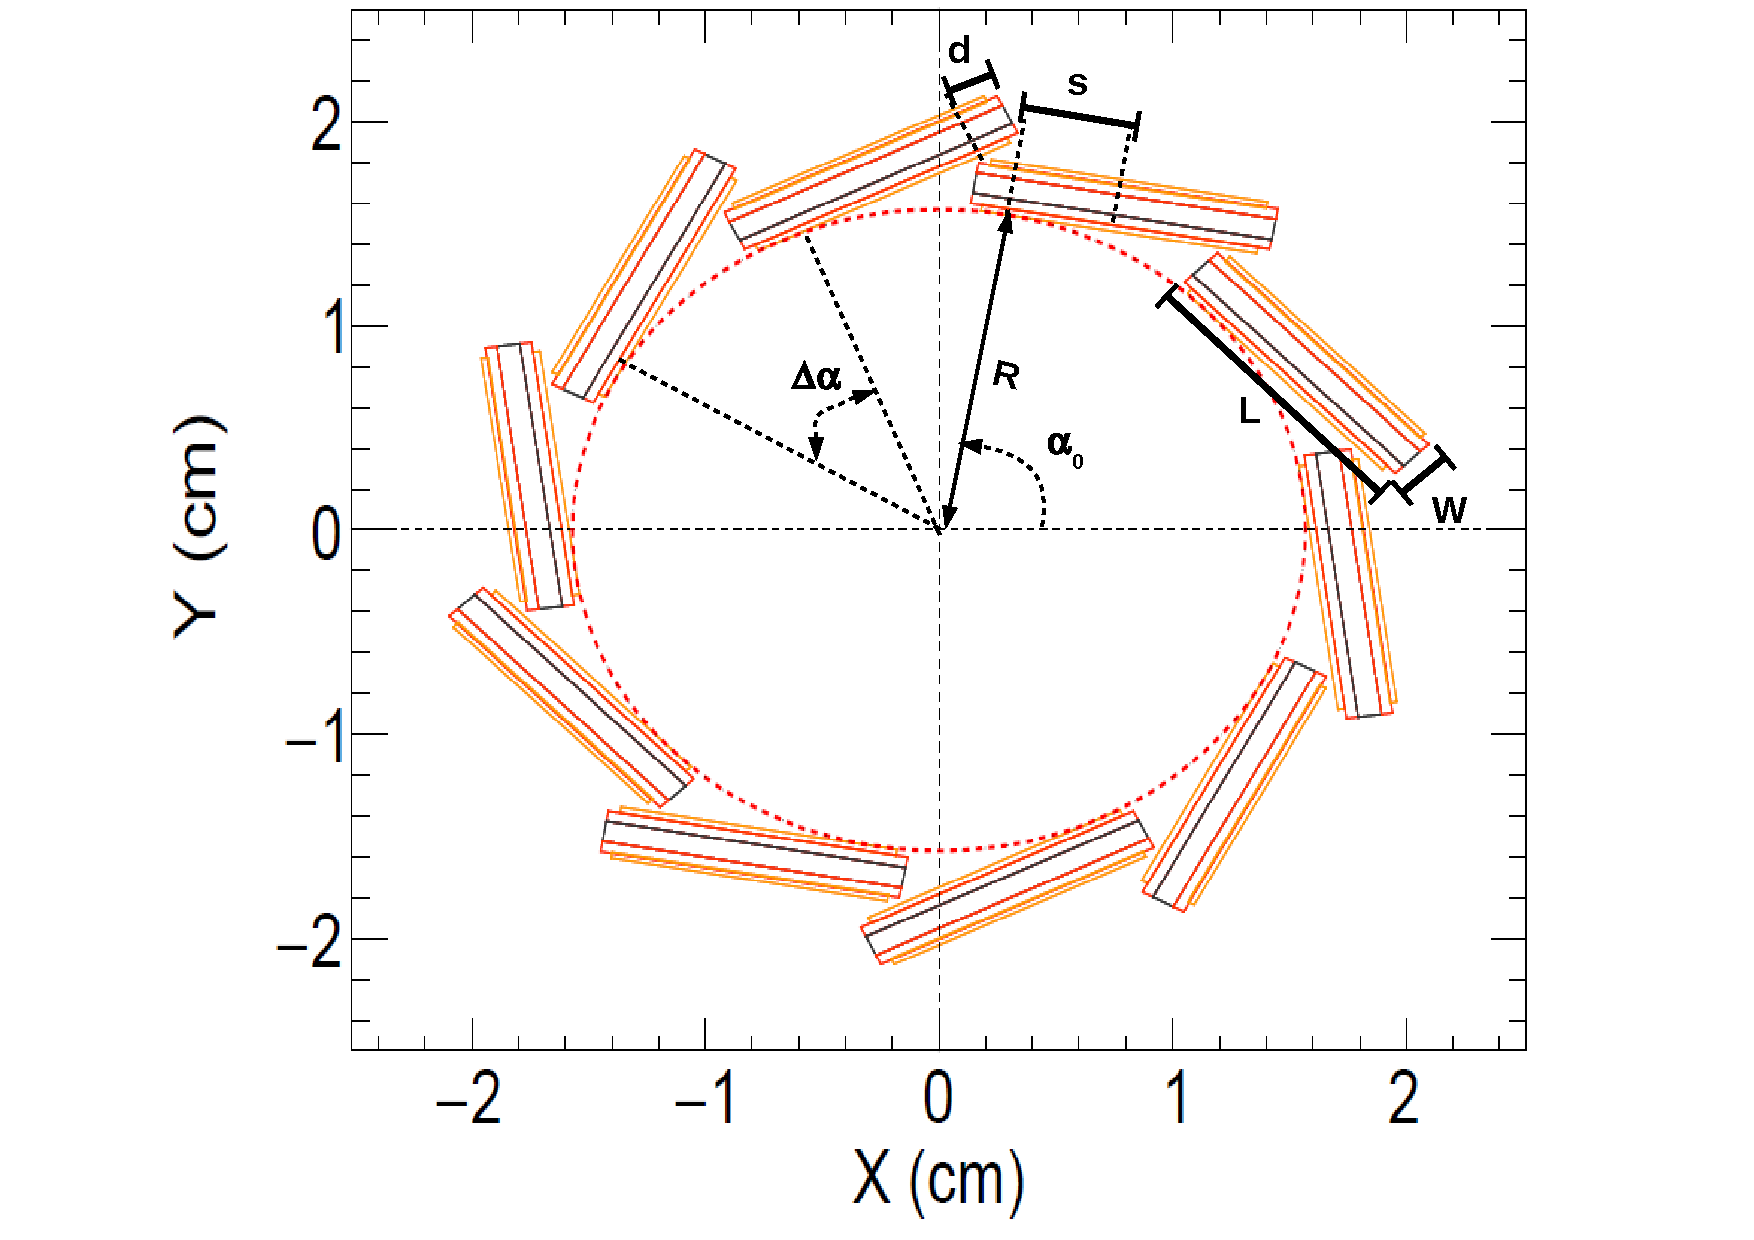
\includegraphics[width=0.9\textwidth]{figures/Spiral_Mosaic.pdf}
  \caption{Spiral plane ladder mosaic configuration.}
  \label{fig:Spiral_Plane_ladder_mosaic}
\end{figure}

\begin{itemize}
 \item  {\bf Spiral configuration}: 
   \begin{eqnarray}
     \label{eq:spiral_overlap}
     \frac{d}{L}   &=& 1 - \left(\frac{1 - \cos(\Delta\alpha)}{\sin(\Delta\alpha)}\right) \left(\frac{w + 2R}{L}\right) \\
     \label{eq:spiral_shift}
     \frac{s}{L}   &=& \left(1 - \frac{d}{L}\right) \left( \frac{R - (R + w)\cos(\Delta\alpha)}{ (1 - \cos(\Delta\alpha))(w + 2R)} \right) \\
     \Delta\alpha  &=& \frac{2\pi}{N_{\rm ladders}}
   \end{eqnarray}
   
   \item  {\bf Alternating configuration}: 
   \begin{eqnarray}
   \label{eq:alternating_overlap}
     \frac{d}{L}   &=& \frac{L(1 + \cos(\Delta\alpha)) - 2(w + R)\sin(\Delta\alpha)}{2L} \\
     \label{eq:alternating_shift}
     \frac{s}{L}   &=& \frac{(1 + w/R) [1 + (1 - 2\frac{d}{L})\cos(\Delta\alpha)]}{1 - 2\frac{d}{L} + \cos(\Delta\alpha)} \\
     \Delta\alpha  &=& \frac{2\pi}{N_{\rm ladders}/2}
   \end{eqnarray}
\end{itemize}
\noindent
Where $N_{\rm ladders}$ is the number of ladders.

\begin{figure}
  \centering
  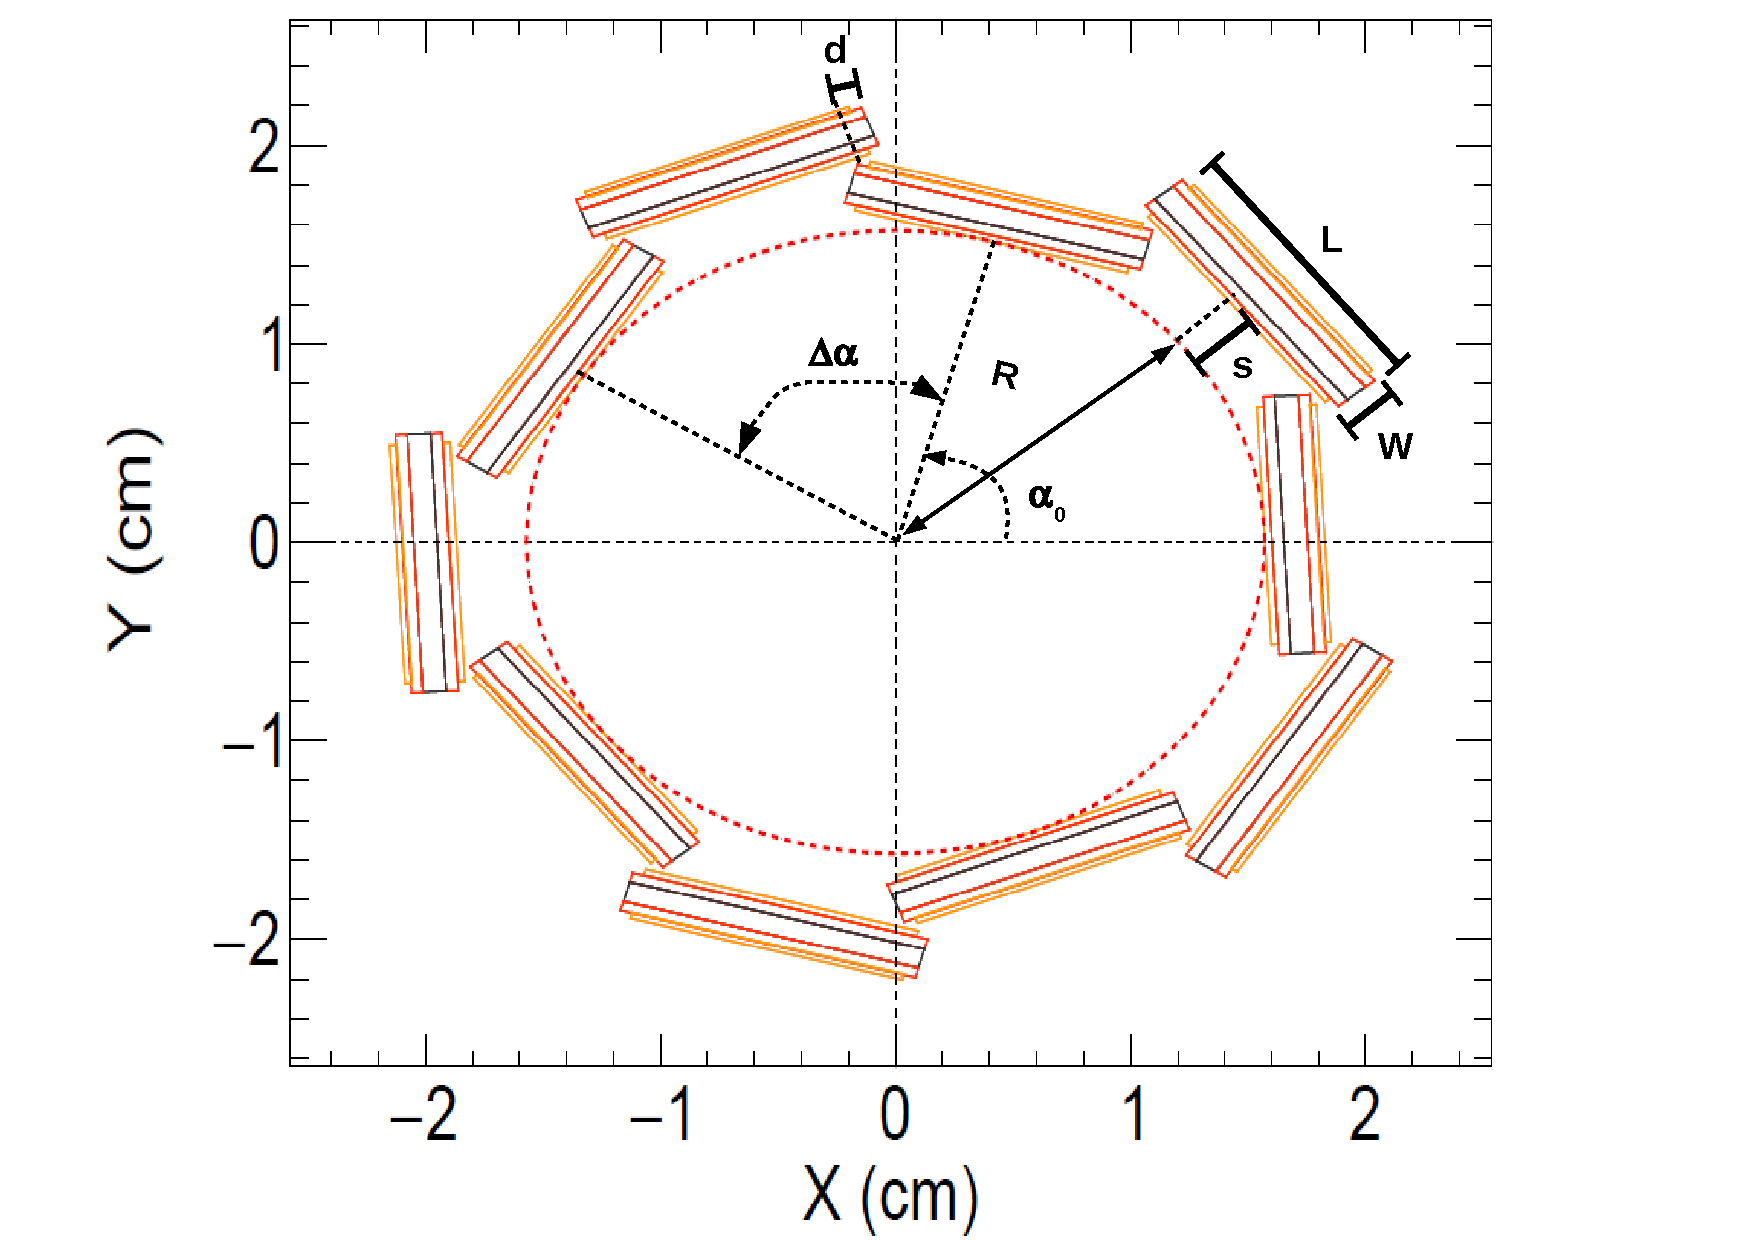
\includegraphics[width=0.9\textwidth]{figures/Alternating_Mosaic.pdf}
  \caption{Alternating plane ladder mosaic configuration.}
  \label{fig:Alternating_Plane_ladder_mosaic}
\end{figure}

~\\
The syntax to specify such structures is as follows.

~\\
\noindent
{\tt BeginMosaicLadderPlane} \\
$~~~~~${\tt LadderName        string                   $~~~~~~~~~~~~$   // (Mandatory)} \\
$~~~~~${\tt LadderMosaic      string                     $~~~~~~~~~~$   // (Mandatory)} \\
$~~~~~${\tt LadderPosition    x  y  z units                     $~~~$   // (Mandatory)} \\
$~~~~~${\tt LadderRotAngles   $\alpha_x$  $\alpha_y$  $\alpha_z$ units  // (Optional)}  \\
$~~~~~${\tt LadderVarPar      string                     $~~~~~~~~~~$   // (Mandatory)} \\
$~~~~~${\tt LadderRadius      value units                    $~~~~~$    // (Mandatory)} \\
$~~~~~${\tt LadderOverlap     value units                    $~~~~~$    // (Mandatory)} \\
$~~~~~${\tt LadderClearanceH  value units                       $~~$    // (Optional)} \\
$~~~~~${\tt LadderClearanceV  value units                       $~~$    // (Optional)} \\
$~~~~~${\tt LadderAlpha0      value units                   $~~~~~~$    // (Optional)} \\
$~~~~~${\tt LadderN           value              $~~~~~~~~~~~~~~~~~$    // (Mandatory)} \\
$~~~~~${\tt LadderShift       value                  $~~~~~~~~~~~~~$    // (Optional)} \\
$~~~~~${\tt LadderShiftFix    bool                      $~~~~~~~~~~~$    // (Optional)} \\
$~~~~~${\tt BeginPlane} \\
$~~~~~~~${\tt Name             string                   $~~~~~~~~~~~~$   // (Mandatory)} \\
$~~~~~~~${\tt Position         x  y  z units                     $~~~$   // (Mandatory)} \\
$~~~~~~~${\tt Thickness        value  units                       $~~$   // (Mandatory, value > 0)} \\
$~~~~~~~${\tt Material         string                       $~~~~~~~~$   // (Mandatory)} \\
$~~~~~~~${\tt XOX0             value                   $~~~~~~~~~~~~~$   // (Optional)}  \\
$~~~~~~~${\tt widthU           value units                     $~~~~~$   // (Mandatory, value > 0)} \\
$~~~~~~~${\tt widthV           value units                     $~~~~~$   // (Mandatory, value > 0)} \\
$~~~~~~~${\tt IsSensitive      bool                          $~~~~~~~$   // (Mandatory)} \\
$~~~~~~~${\tt ResolutionU      value units                               // (Optional, value > 0)} \\
$~~~~~~~${\tt ResolutionV      value units                               // (Optional, value > 0)} \\
$~~~~~~~${\tt Resolution       value units                               // (Optional, value > 0)} \\
$~~~~~~~${\tt ROtime           value units                      $~~~~$   // (Optional, value > 0)} \\
$~~~~~~~${\tt Efficiency       value                          $~~~~~~$   // (Optional, 0 <= value <= 1)} \\
$~~~~~~~${\tt InsensFracVneg   value                              $~~$   // (Optional, default is zero)} \\
$~~~~~~~${\tt InsensFracVpos   value                              $~~$   // (Optional, default is zero)} \\
$~~~~~~~${\tt BkgRate          value units                       $~~~$   // (Optional, default is zero)} \\
$~~~~~~~${\tt SystemName       string                          $~~~~~$   // (Optional)} \\
$~~~~~~~${\tt LayerName        string                         $~~~~~~$   // (Optional)} \\
$~~~~~~~${\tt ResolutionModel  string                                    // (Optional)} \\
$~~~~~~~${\tt EfficiencyModel  string                                    // (Optional)} \\
$~~~~~${\tt EndPlane} \\
$~~~~~$ ... \\
{\tt EndMosaicLadderPlane}

~\\
As in the case of the plane ladder, an indefinite number of planes can be specified. Out of this list the system
will calculate $L$ and $w$ (see figures~\ref{fig:Spiral_Plane_ladder_mosaic} and~\ref{fig:Alternating_Plane_ladder_mosaic}) 
as the maximum width and total thickness of the ladder adding a clearance of {\tt LadderClearanceH} and {\tt LadderClearanceV}, 
respectively. The {\tt LadderMosaic} parameter defines the type of structure to build, it can only have the values "Spiral" or 
"Alternating". Another important parameter is {\tt LadderVarPar}, which is the parameter to be calculated out of the others using 
Eq.~\ref{eq:spiral_overlap} or~\ref{eq:alternating_overlap}. This parameter can have either the value "Overlap" or "Radius". 
In the first (second) case the overlap $d/L$ (radius $R$) is calculated fixing all the other parameters. The shift $s/L$ is 
then calculated from Eq~\ref{eq:spiral_shift} or~\ref{eq:alternating_shift}. If the boolean parameter {\tt LadderShiftFix} is set 
to {\tt true}, the shift will be fixed to the specified value {\tt LadderShift}.

\subsubsection{Petal ladder mosaic}

A petal ladder mosaic is complex structure made from petal ladders to resemble a disk as shown in figure~\ref{fig:Petal_ladder_mosaic}.
The syntax to specify such structure is as follows.

~\\
\noindent
{\tt BeginMosaicLadderPetal} \\
$~~~~~${\tt LadderName        string                   $~~~~~~~~~~~~$   // (Mandatory)} \\
$~~~~~${\tt LadderPosition    x  y  z units                     $~~~$   // (Mandatory)} \\
$~~~~~${\tt LadderRotAngles   $\alpha_x$  $\alpha_y$  $\alpha_z$ units  // (Optional)}  \\
$~~~~~${\tt LadderRadius      value units                    $~~~~~$    // (Mandatory)} \\
$~~~~~${\tt LadderAlpha0      value units                   $~~~~~~$    // (Optional)} \\
$~~~~~${\tt LadderN           value              $~~~~~~~~~~~~~~~~~$    // (Mandatory)} \\
$~~~~~${\tt LadderShift       value units                  $~~~~~~~$    // (Optional)} \\
$~~~~~${\tt BeginPetal} \\
$~~~~~~~${\tt Name             string                   $~~~~~~~~~~~~$   // (Mandatory)} \\
$~~~~~~~${\tt Position         x  y  z units                     $~~~$   // (Mandatory)} \\
$~~~~~~~${\tt Thickness        value  units                       $~~$   // (Mandatory, value > 0)} \\
$~~~~~~~${\tt Material         string                       $~~~~~~~~$   // (Mandatory)} \\
$~~~~~~~${\tt XOX0             value                   $~~~~~~~~~~~~~$   // (Optional)}  \\
$~~~~~~~${\tt bottomWidth      value units                               // (Mandatory, value > 0)} \\
$~~~~~~~${\tt topWidth         value units                       $~~~$   // (Mandatory, value > 0)} \\
$~~~~~~~${\tt Height           value units                     $~~~~~$   // (Mandatory, value > 0)} \\
$~~~~~~~${\tt IsSensitive      bool                          $~~~~~~~$   // (Mandatory)} \\
$~~~~~~~${\tt ResolutionU      value units                               // (Optional, value > 0)} \\
$~~~~~~~${\tt ResolutionV      value units                               // (Optional, value > 0)} \\
$~~~~~~~${\tt Resolution       value units                               // (Optional, value > 0)} \\
$~~~~~~~${\tt ROtime           value units                      $~~~~$   // (Optional, value > 0)} \\
$~~~~~~~${\tt Efficiency       value                          $~~~~~~$   // (Optional, 0 <= value <= 1)} \\
$~~~~~~~${\tt InsensFracVneg   value                              $~~$   // (Optional, default is zero)} \\
$~~~~~~~${\tt InsensFracVpos   value                              $~~$   // (Optional, default is zero)} \\
$~~~~~~~${\tt BkgRate          value units                       $~~~$   // (Optional, default is zero)} \\
$~~~~~~~${\tt SystemName       string                          $~~~~~$   // (Optional)} \\
$~~~~~~~${\tt LayerName        string                         $~~~~~~$   // (Optional)} \\
$~~~~~~~${\tt ResolutionModel  string                                    // (Optional)} \\
$~~~~~~~${\tt EfficiencyModel  string                                    // (Optional)} \\
$~~~~~${\tt EndPetal} \\
$~~~~~$ ... \\
{\tt EndMosaicLadderPetal}

~\\
As in the case of the plane ladder, an indefinite number of petals can be specified taking care that they not overlap. 
In figure~\ref{fig:Petal_ladder_mosaic} can be appreciated the parameters needed to build this structure. {\tt LadderRadius} 
is $R$, {\tt LadderAlpha0} is $\alpha_0$, and {\tt LadderN} is half the number of petals. The {\tt LadderShift} parameter in 
this case is a shift along the disk normal vector. The petals marked by "$+$" ("$-$") in figure~\ref{fig:Petal_ladder_mosaic}
are shifted by $+${\tt LadderShift} ($-${\tt LadderShift}) along this direction.

\begin{figure}
  \centering
  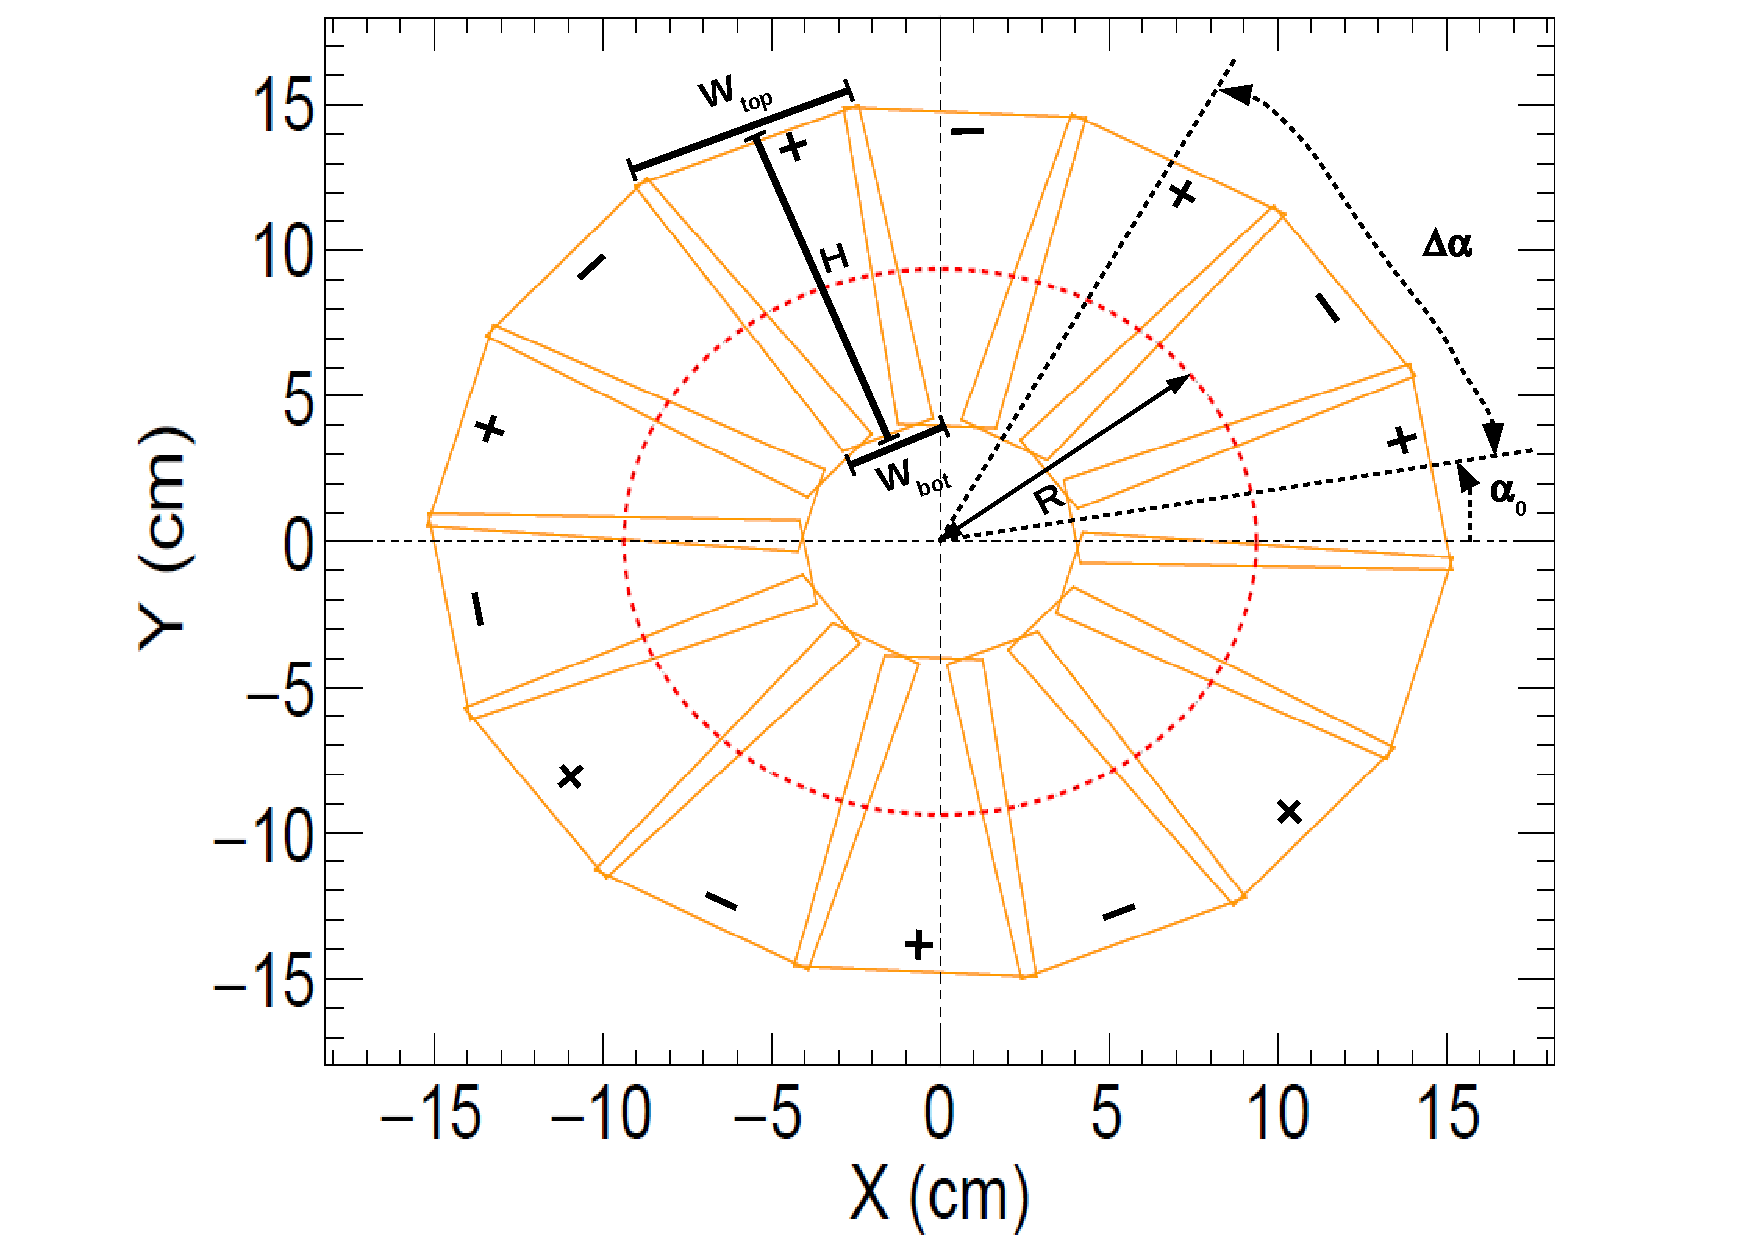
\includegraphics[width=0.9\textwidth]{figures/Petal_Mosaic.pdf}
  \caption{Petal ladder mosaic configuration.}
  \label{fig:Petal_ladder_mosaic}
\end{figure}

~\\
~\\
\noindent
This completes the kind of geometrical structures that can be build in {\guari}. 

\subsection{Intrinsic resolution model}

By default in {\guari} the spatial resolution of any measurement is equal to the intrinsic resolution ({\tt ResolutionU/V}) of the sensitive element. 
Moreover, the spatial resolution of a sensor could depend as well on the intersection coordinates and momentum with the sensor's main surface, and on 
some other parameters. This is a reason behind of the resolution model.

\subsubsection{Gas detector resolution model}
\label{subsubsec:GasDet_resolModel}

For the moment there is only one resolution model implemented, mainly to model the spatial resolution of gas detectors as a TPC or a drift-chamber. 
The syntax is as follows.

~\\
\noindent
{\tt BeginTPCResolutionModel} \\
$~~~~~${\tt Name        string                    $~~~~~~~~~~~$    // (Mandatory)} \\
$~~~~~${\tt A\_U         value units                  $~~~~~~~$    // (Mandatory, value > 0)} \\
$~~~~~${\tt B\_U         value units                  $~~~~~~~$    // (Mandatory, value > 0)} \\
$~~~~~${\tt C\_U         value units                  $~~~~~~~$    // (Mandatory, value > 0)} \\
$~~~~~${\tt A\_V         value units                  $~~~~~~~$    // (Mandatory, value > 0)} \\
$~~~~~${\tt B\_V         value units                  $~~~~~~~$    // (Mandatory, value > 0)} \\
{\tt EndTPCResolutionModel}

~\\
The {\tt Name} parameter defines the resolution model. Any sensor with its parameter {\tt ResolutionModel} set 
to this name will use this resolution model. The resolution is calculated as follows,

\begin{eqnarray}
  {\rm ResolutionU}^2 &=& {\rm A_U}^2 + {\rm B_U}^2\sin\phi + {\rm C_U}\sin\theta\times z, \\
  {\rm ResolutionV}^2 &=& {\rm A_V}^2 + {\rm B_V}\times z;
\end{eqnarray}
\noindent
where $\theta$, $\phi$ and $z$ are the polar and azimuthal angles of the momentum and the z-coordinate at the intersection of the track with 
the volume main surface.

~\\
\noindent
See section~\ref{subsubsec:Example3} for an example illustrating of this resolution model.

\subsection{Detection efficiency model}

As in the case of the spatial resolution, by default in {\guari} the detection efficiency of any measurement is equal to the intrinsic detection efficiency ({\tt Efficiency}) 
of the sensitive element. Moreover, the detection efficiency of a sensor could depend as well on the intersection coordinates and momentum with the sensor's main surface, and 
on some other parameters. This is a reason behind of the efficiency model.

~\\
~\\
\noindent
For the time being there is no Efficiency model implemented in {\guari}, only a base class.

\subsection{Systems configuration}

It is useful to label a set of geometry elements as a system. The usefulness has already being shown the examples of 
sections~\ref{subsubsec:Example2} and ~\ref{subsubsec:Example4}, for the material budget studies. The syntax to define the 
systems configurations is as follows.

~\\
\noindent
{\tt BeginSystemsConfiguration} \\
$~~~~~${\tt BeginSystem} \\
$~~~~~~~${\tt Name             string       $~~~~~~~~~~~~~~~~~~~~$   // (Mandatory)} \\
$~~~~~~~${\tt LayersList       string1  string2  ....                // (Mandatory)} \\
$~~~~~${\tt EndSystem} \\
$~~~~~$ ... \\
{\tt EndSystemsConfiguration}

~\\
\noindent
where {\tt LayerList} is a list of geometry element {\tt LayerName}. The user can define as many systems as needed, but 
no two systems can share the same {\tt LayerName}.

\subsection{Telescope-DUT configuration}
\label{subsec::TelDUT_config}

In some cases it is interesting to understand the pointing precision of tracks reconstructed with a set of sensitive elements (Telescope) 
toward some other elements (DUTs). The use of this feature has been illustrated in examples of sections~\ref{subsubsec:Example1} and ~\ref{subsubsec:Example2}.
The syntax for configuring a Telescope-DUT setup is as follows.

~\\
\noindent
{\tt BeginBeamTestConfiguration} \\
$~~~~~${\tt TelescopeLayersList  string1   string2  string3  ... // (Mandatory)} \\
$~~~~~${\tt DUTLayersList        string1   string2  string3  ... $~~~~~$ // (Mandatory)} \\
{\tt EndBeamTestConfiguration}

~\\
\noindent
where {\tt TelescopeLayersList} and {\tt DUTLayersList} are lists with the {\tt LayerName}s which define the Telescope and DUTs, respectively.

\subsection{Track-Finder algorithms}
\label{subsec::TrkFinder_config}

When calculating the tracking efficiency a co-called {\tt TrackFinderAlgo} object has to be specified. Each such object will be used 
for a certain regions of the tracker. No two {\tt TrackFinderAlgo} can have overlapping regions, in such a case the program will crash with 
an error message.

For the time being only one track-finder object has been implemented, the so-called FPCCDTrackFinderAlgo. Its syntax is described in the section 
below.

\subsubsection{FPCCD Track-Finder algorithm}

The syntax for this track finder is as follows,

~\\
\noindent
{\tt BeginFPCCDTrackFinderAlgo}
$~~~~~${\tt Name              string                (Mandatory)} \\
$~~~~~${\tt PtMin             val units // val > 0  (Mandatory)} \\
$~~~~~${\tt NhitsMin          val       // val > 0  (Mandatory)} \\
$~~~~~${\tt PurityMin         val       // val > 0  (Optional, default value is 1)} \\
$~~~~~${\tt Chi2OndfSeed      val       // val > 0  (Optional, default value is 3)} \\
$~~~~~${\tt Chi2OndfAdd       val       // val > 0  (Optional, default value is 3)} \\
$~~~~~${\tt NfakesMaxSeeding  val       // val >= 0 (Optional, default value is 0)} \\
$~~~~~${\tt NmcSeedEffic      val       // val >= 0 (Optional, default value is 1000)} \\
$~~~~~${\tt BeginTrackFinderRegion} \\
$~~~~~~~${\tt positionRangeX      min  max  units // max > min (Optional)} \\
$~~~~~~~${\tt positionRangeY      min  max  units // max > min (Optional)} \\
$~~~~~~~${\tt positionRangeZ      min  max  units // max > min (Optional)} \\
$~~~~~~~${\tt positionRangeR      min  max  units // max > min (Optional)} \\
$~~~~~~~${\tt positionRangeTheta  min  max  units // max > min (Optional)} \\
$~~~~~~~${\tt positionRangePhi    min  max  units // max > min (Optional)} \\
$~~~~~~~${\tt momentumRangeP      min  max  units // max > min and both >= 0 (Optional)} \\
$~~~~~~~${\tt momentumRangeTheta  min  max  units // max > min (Optional)} \\
$~~~~~~~${\tt momentumRangePhi    min  max  units // max > min (Optional)} \\
$~~~~~${\tt EndTrackFinderRegion} \\
$~~~~~${\tt BeginSystems} \\
$~~~~~~~${\tt System   string} \\
$~~~~~~~${\tt ...} \\
$~~~~~${\tt EndSystems} \\
$~~~~~${\tt BeginSeedConfigs} \\
$~~~~~~~${\tt SeedConfig   string1  string2  string3 ...} \\
$~~~~~~~${\tt ...} \\
$~~~~~${\tt EndSeedConfigs} \\
{\tt EndFPCCDTrackFinderAlgo}

~\\
\noindent
where 

\begin{itemize}
  \item  {\tt PtMin} is the $p^{\rm min}_t$ cut for seeding.
  
  \item  {\tt NhitsMin} is the minimum number of hits allowed to reconstruct the track.
  
  \item  {\tt PurityMin} is the minimum allowed value of the track purity, defined as (\# good hits)/(\# hits). It defined the maximum number of 
  fake hits in the track as follows, $N^{\rm max}_{\rm fake} = N_{hit}(1 - {\rm PurityMin})$.

  \item  {\tt Chi2OndfSeed} is the $(\chi^2/ndf)_{\rm max}$ for seed tracks.
  
  \item  {\tt Chi2OndfAdd} is the $\chi^2/ndf$ maximum cut for track-hit association.
  
  \item  {\tt NfakesMaxSeeding} is the maximum allowed number of fake hits for seeding.
  
  \item  {\tt NmcSeedEffic} is the number of samplings for the seeding efficiency MC calculation.
\end{itemize}

The region where this {\tt TrackFinderAlgo} object will be used is specified in the block between {\tt BeginTrackFinderRegion} and 
{\tt EndTrackFinderRegion}. The region is specified in terms of the track origin and momentum. At least of the possible ranges has to be specified.

The systems considered for the tracking is specified in the block between {\tt BeginSystems} and {\tt EndSystems}. Each entry in this block 
should be the full system name ({\tt SystemName}).

Finally, the seeding configurations are specified in the block between {\tt BeginSeedConfigs} and {\tt EndSeedConfigs}. Every seed 
configuration is specified by listing sets of three layer-names ({\tt LayerName}).

~\\
\noindent
See section~\ref{subsubsec:FPCCDTrkEffic_calculation} for a detailed explanation of the parameters above as well as the process for the tracking efficiency calculation.

\subsection{Track cuts}

In some cases it is needed to perform cuts on the number of hits within a system for tracks in some ranges of its momentum components $(p,\theta,\phi)$. 
The syntax is as follows.

~\\
\noindent
{\tt BeginTrackCuts} \\
$~~~~~${\tt SystemName        string        $~~~~~~~$   // (Mandatory)} \\
$~~~~~${\tt BeginCut} \\
$~~~~~~~${\tt pRange           min  max  units  $~~~$   // (Optional)} \\
$~~~~~~~${\tt phiRange         min  max  units    $~$   // (Optional)} \\
$~~~~~~~${\tt thetaRange       min  max  units          // (Optional)} \\
$~~~~~~~${\tt NhitsRange       min  max  units          // (Mandatory)} \\
$~~~~~${\tt EndCut} \\
$~~~~~$ ... \\
{\tt EndTrackCuts}

~\\
\noindent
Where SystemName is the name of the system in which the cut on the number of hits will be applied. The data structure between {\tt BeginCut} and {\tt EndCut} 
implement the cut. The $p$, $\theta$ and $\phi$ ranges ({\tt pRange}, {\tt phiRange} and {\tt thetaRange}, respectively) identify the range of momentum where the 
cut {\tt NhitsRange} will be applied. While implementing a cut, at least one range, either $p$, $\theta$ or $\phi$ range has to be specified.

\subsection{Global hit rate scaling}
\label{subsec:global_bkgrate_scaling}

This is a feature is for globally scaling the hit rates on all the sensitive elements of the geometry. This could be useful to study tracking performances 
in terms of the hit rate labels. The syntax for this feature is very simple.

~\\
\noindent
{\tt GlobalBkgRateScaling:  scaling} \\

~\\
\noindent
where the {\tt scaling} has to be $\geq 0$. If not the program will crash with an error message.

~\\
~\\
\noindent
This concludes all what is needed to build a geometry. Lets now continue to the next section where the analysis configurations will be described.


\section{Analysis configuration}
\label{sec:analysis_config}

In this section is described the syntax for the main data-card file. The items below describe general parameters for all the analysis which are either mandatory or optional. 
Later sections will describe the syntax to setup the different analysis. See section~\ref{subsec:Some_examples} for some examples illustrating this features.

\begin{itemize}
 \item  {\bf Verbosity}: the {\tt Verbose:} parameter is a boolean optional parameter (default value is false). It is a flag used for debugging. 
 If true is several print-outs will be displayed.

 \item  {\bf Particle parameters}:
 \begin{itemize}
   \item {\tt ParticleType:} a mandatory parameter. Possible values is the list of stable particles: {\tt e-} or {\tt e+} (electron/positron), 
   {\tt mu+} or {\tt mu-} (muon), {\tt pi+} or {\tt pi-} (pion), {\tt K+} or {\tt K-} (Kaon), {\tt p+} or {\tt p-} (proton), {\tt 4He++} (double-ionized Helium-4).
   
   \item  {\tt ParticleOrigin:} a mandatory parameter. It is the point $(x,y,z)$ from which the particle is going to be tracker in the process of
   geometry navigation.
 \end{itemize}
   
 \item  {\bf Pivot point}: {\tt ReferencePoint} is a mandatory parameter. Trajectories are always parameterized in terms of some quantities defined with respect to
 a pivot-point.
 
 \item  {\bf MC seed}: {\tt MCSeed:} is an optional parameter. This seed is used to initialize the random-generator used for the MC calculation of the seeding 
 efficiency (c.f. sec.~\ref{subsubsec:FPCCDTrkEffic_calculation}).
 
 \item  {\bf Include $E_{\rm loss}$ calculation}: the {\tt IncludeEloss:} parameter is a boolean optional parameter (default value is true). It is a flag used for including 
 the $E_{\rm loss}$ fluctuations in the measurements covariance matrix (c.f. sec.~\ref{subsec:TrkParm_CovMatrix_calculation}).
 
 \item  {\bf Tunning the $E_{\rm loss}$ fluctuations model}: the $\kappa$ parameter in the $E_{\rm loss}$ fluctuations model (c.f. eq.~\ref{eq:sigmaEloss}) can be modified if needed 
 with the following syntax,
 
 ~\\
 \noindent     
 {\tt KappaElossFluctuation:  value units} \\
 ~\\
 \noindent
 where the units should be those of energy.
 
 
 \item {\bf The momentum scan parameters}: a set of values for the momentum or energy variable (see below), polar variable ($\theta$, $\cos\theta$ or $\eta$) and azimuthal angle ($\phi$). 
 All of them can be specified as a range or as a set of discrete values. Here below are the possibilities
 \begin{itemize}
   \item {\bf Momentum or energy variable}: the momentum or energy variable can be specified in four ways, either $p$ (momentum), $E$ (energy), $E_{kin}$ (kinetic energy) or $E_{kin}/u$ 
   (kinetic energy per nucleon); where the last one is only useful when studying ionized heavy nuclei. For each of them the either a list of discrete values or 
   a range can be specified. The syntax for all these possibilities is as follows,
   
   \begin{itemize}
     \item {\bf List of discrete momentum values}:
     
     \noindent
     {\tt MomentumValues: value1  value2  value3 ... units } \\
     \noindent
     where as many values as needed can be specified. At least one value needs to be specified.
     ~\\
     
     \item {\bf Momentum range}: syntax is as follows,
     ~\\
     \noindent     
     {\tt BeginMomentumScan} \\
     $~~~~${\tt Nbins   integer $~~$ // (Mandatory)} \\
     $~~~~${\tt pMin    value units  // (Mandatory)} \\
     $~~~~${\tt pMax    value units  // (Mandatory)} \\
     {\tt EndMomentumScan}
     ~\\
     
     \item {\bf List of discrete energy values}:
     
     \noindent
     {\tt EnergyValues: value1  value2  value3 ... units } \\
     \noindent
     where as many values as needed can be specified. At least one value needs to be specified.
     ~\\
     
     \item {\bf Energy range}: syntax is as follows,
     ~\\
     \noindent     
     {\tt BeginEnergyScan} \\
     $~~~~${\tt Nbins   integer $~~$ // (Mandatory)} \\
     $~~~~${\tt EMin    value units  // (Mandatory)} \\
     $~~~~${\tt EMax    value units  // (Mandatory)} \\
     {\tt EndEnergyScan}
     ~\\
     
     \item {\bf List of discrete kinetic energy values}:
     
     \noindent
     {\tt EkinValues: value1  value2  value3 ... units } \\
     \noindent
     where as many values as needed can be specified. At least one value needs to be specified.
     ~\\
     
     \item {\bf Kinetic energy range}: syntax is as follows,
     ~\\
     \noindent     
     {\tt BeginEkinScan} \\
     $~~~~${\tt Nbins   integer $~~$ // (Mandatory)} \\
     $~~~~${\tt EkinMin    value units  // (Mandatory)} \\
     $~~~~${\tt EkinMax    value units  // (Mandatory)} \\
     {\tt EndEkinScan}
     ~\\
     
     \item {\bf List of discrete kinetic energy per nucleon values}:
     
     \noindent
     {\tt EkinPerUValues: value1  value2  value3 ... units } \\
     \noindent
     where as many values as needed can be specified. At least one value needs to be specified.
     ~\\
     
     \item {\bf Kinetic energy per nucleon range}: syntax is as follows,
     ~\\
     \noindent     
     {\tt BeginEkinPerUScan} \\
     $~~~~${\tt Nbins   integer $~~$ // (Mandatory)} \\
     $~~~~${\tt EkinPerUMin    value units  // (Mandatory)} \\
     $~~~~${\tt EkinPerUMax    value units  // (Mandatory)} \\
     {\tt EndEkinPerUScan}
     ~\\
     
   \end{itemize}
   If no $p$, $E$, $E_{kin}$ or $E_{kin}/u$ values are specified, then a single $p = 2~{\rm GeV/c}$ value will be will be used. Non of the momentum or energy values can be negative, if so the program will 
   crash with an error message. Furthermore, in the case of specifying energy values, $E$, all the specified values have to be larger than the particle mass, otherwise the program will crass with an error 
   message.
   ~\\
 
   \item {\bf Polar variable}: the polar variable can be specified in three ways, either $\theta$, $\cos\theta$ or $\eta$. For each of them the either a list of discrete values or 
   a range can be specified. The syntax for all these possibilities is as follows,
   
   \begin{itemize}
     \item {\bf List of discrete $\theta$ values}:
     
     \noindent
     {\tt PolarAngleValues: value1  value2  value3 ... units } \\
     \noindent
     where as many values as needed can be specified. At least one value needs to be specified.
     ~\\
     
     \item {\bf $\theta$ Range}:
     ~\\
     \noindent     
     {\tt BeginPolarAngleScan} \\
     $~~~~${\tt Nbins       integer $~~~~~~$ // (Mandatory)} \\
     $~~~~${\tt thetaMin    value units      // (Mandatory)} \\
     $~~~~${\tt thetaMax    value units      // (Mandatory)} \\
     {\tt EndPolarAngleScan}
     ~\\
     
     \item {\bf List of discrete $\cos\theta$ values}:
     
     \noindent
     {\tt CosThetaValues: value1  value2  value3 ... units } \\
     \noindent
     where as many values as needed can be specified. At least one value needs to be specified.
     ~\\
     
     \item {\bf $\cos\theta$ Range}:
     ~\\
     \noindent     
     {\tt BeginCosThetaScan} \\
     $~~~~${\tt Nbins          integer $~~~~~~~~~$ // (Mandatory)} \\
     $~~~~${\tt costhetaMin    value units         // (Mandatory)} \\
     $~~~~${\tt costhetaMax    value units         // (Mandatory)} \\
     {\tt EndCosThetaScan}
     ~\\
     
     \item {\bf List of discrete $\eta$ values}:
     
     \noindent
     {\tt EtaValues: value1  value2  value3 ... units } \\
     \noindent
     where as many values as needed can be specified. At least one value needs to be specified.
     ~\\
     
     \item {\bf $\eta$ Range}:
     ~\\
     \noindent     
     {\tt BeginEtaScan} \\
     $~~~~${\tt Nbins     integer $~~~~$ // (Mandatory)} \\
     $~~~~${\tt etaMin    value units         // (Mandatory)} \\
     $~~~~${\tt etaMax    value units         // (Mandatory)} \\
     {\tt EndEtaScan}
     ~\\
     
   \end{itemize}
   
   \item {\bf Azimuthal angle}: 
   \begin{itemize}
     \item {\bf List of discrete values}: syntax is as follows,
     
     \noindent
     {\tt AzimuthalAngleValues: value1  value2  value3 ... units } \\
     \noindent
     where as many values as needed can be specified. At least one value needs to be specified.
     
     \item {\bf Range}: syntax is as follows,
     ~\\
     \noindent     
     {\tt BeginAzimuthalAngleScan} \\
     $~~~~${\tt Nbins     integer $~~~~$ // (Mandatory)} \\
     $~~~~${\tt phiMin    value units    // (Mandatory)} \\
     $~~~~${\tt phiMax    value units    // (Mandatory)} \\
     {\tt EndAzimuthalAngleScan}
   \end{itemize}
   
 \end{itemize}
 
 \item {\bf Momentum resolution representation}: In the case where $p$ or $p_{t}$ is part of the track parameters, its resolution can be 
 represented in different ways: $\sigma(p)/p$, $\sigma(p)$ or $\sigma(1/p)$. The default one is $\sigma(p)/p$. A parameter allows to select the 
 representation as {\tt MonResolRepresentation: string}, where {\tt string} can only have the values: {\tt sigma(Pt)/Pt}, {\tt sigma(Pt)} or 
 {\tt sigma(1/Pt)}, corresponding to the $\sigma(p)/p$, $\sigma(p)$ or $\sigma(1/p)$ representations, respectively.
 
 \item {\bf Geometry list}: the list of geometries is specified as follows,
 
 \noindent
 {\tt BeginGeometries} \\
 $~~~~${\tt fullpath/geo-data-card1.txt} \\
 $~~~~${\tt fullpath/geo-data-card2.txt} \\
 $~~~~${\tt ...} \\
 {\tt EndGeometries}
 
 \noindent
 where {\tt fullpath} is the full path of the location of the geo-data-card. The user can specify as many geometries as needed. At least one 
 geometry needs to be specified, otherwise the program will crash with an error message.
 
 \item {\bf Ranges for geometry visualization}: as a default a geometry will be visualized in a range on $X$, $Y$ and $Z$ that contain all the geometry elements. It is possible to 
 specify a set of sub-ranges for a better appreciation of the geometry. This can be made as follows,
 
 \noindent
 {\tt BeginGeoRanges} \\
 $~~~~${\tt BeginRange} \\
 $~~~~~~~${\tt XRange   min  max units} \\
 $~~~~~~~${\tt YRange   min  max units} \\
 $~~~~~~~${\tt ZRange   min  max units} \\
 $~~~~${\tt EndRange} \\
 $~~~~${\tt ...} \\
 {\tt EndGeoRanges}
 
 \noindent
 As many ranges as needed can be specified. At least one of the {\tt XRange}, {\tt YRange} or {\tt ZRange} parameters have to be specified. For example, if only the 
 {\tt ZRange} is specified, the other two will be set equal to a high range.

 \item {\bf Voxeling}: this is a feature that allows to reduce the computation time in cases where it is known beforehand the regions of the geometry where the particles 
 will pass through. It mainly consist in defining a set of regions. For each specified geometry, a sub-list of geometry elements will be built consisting of those contained 
 in the specified regions. This sub-list will then be used for the calculation of the track-geometry intersections. An illustration of its usage can be found in the example 
 section~\ref{subsubsec:Example3}. The syntax is as follows,
 
 \noindent
 {\tt BeginVoxeling} \\
 $~~~~${\tt BeginVoxel} \\
 $~~~~~~~${\tt xRange       min  max units} \\
 $~~~~~~~${\tt yRange       min  max units} \\
 $~~~~~~~${\tt zRange       min  max units} \\
 $~~~~~~~${\tt rRange       min  max units} \\
 $~~~~~~~${\tt thetaRange   min  max units} \\
 $~~~~~~~${\tt phiRange     min  max units} \\
 $~~~~${\tt EndVoxel} \\
 $~~~~${\tt ...} \\
 {\tt EndVoxeling}
 
 \noindent
 As many voxels as needed can be specified. At least one of the {\tt xRange}, {\tt yRange} or {\tt zRange}, or the polar-coordinates equivalent, {\tt rRange}, {\tt thetaRange} or {\tt phiRange}, 
 parameters have to be specified. For example, if only the {\tt zRange} is specified, the other two will be set equal to a high range.
 
 \item {\bf Output file generic name}: this a mandatory parameter which is specified in the following  way {\tt OutputFile: fullpath/outfile}, where {\tt fullpath} is the location where the output file will be 
 written. The output files, either {\tt .pdf} or {\tt .root} will be named as {\tt fullpath/outfile.pdf} and {\tt fullpath/outfile.root}, respectively. If the {\tt fullpath} directory doesn't exist 
 it will be created.
 
 \item {\bf Save output in a .root file}: the output from all the analysis turned on can be saved in a {\tt .root} file by setting the boolean parameter {\tt SavePlots:} to {\tt true} (default value 
 is {\tt false}).
 
\end{itemize}

The set of configuration parameters described above are generic for all the analyses. In the sections below is described how to configure the different analyses.

\subsection{Geometry visualization analysis}
\label{subsec:GeoVisual_analysis}

All the examples in section~\ref{subsec:Some_examples} have illustrated the geometry visualization feature of the package. There are several parameters to set this up.

\begin{itemize}
  \item  {\bf Geometry printout}: this can be turned on by setting the boolean parameter {\tt PrintGeometry:} to {\tt true} (default value is {\tt false}). If set to {\tt true} a printout 
  of all the specified geometries will be made.
  
  \item  {\bf Geometry weights printout}: this can be turned on by setting the boolean parameter {\tt PrintGeometryWeight:} to {\tt true} (default value is {\tt false}). If set to {\tt true}
  a printout of weights all the specified geometries will be made with a separation by system.
  
  \item  {\bf Geometry plotting}: this can be turned on by setting the boolean parameter {\tt PlotGeometry:} to {\tt true} (default value is {\tt false}). By default a projection of the 
  geometry on the $Z-Y$, $Z-X$ and $X-Y$ will be plotted. Additional features can be turned on in the following way,
  
  \begin{itemize}
    \item  {\bf World volume plotting}: this can be turned on by setting the boolean parameter {\tt PlotWorldVolume:} to {\tt true} (default value is {\tt false}). The world volume will 
    be represented by a set of dotted-red lines.
    
    \item {\bf R-Z geometry projection}: this feature is only useful for geometries with cylindrical symmetry with respect to z-axis. It can be turned on by setting the boolean parameter 
    {\tt DoRZGeoRepresentation:} to {\tt true} (default value is {\tt false}).
    
    \item {\bf Plotting some tracks}: this is an useful feature to understand which geometry elements the track will intersect, for a given initial particle origin and momentum. It can be turned on 
    by setting the the boolean parameter {\tt PlotSomeTracks:} to {\tt true} (default value is {\tt false}). This feature turns on the plotting of a set of trajectories along with its intersections with 
    the geometry. For each specified $(\theta,\phi)$ values, a number of trajectories corresponding to some values of momentum will be plotted. By default, 10 momentum values uniformly spaced between the 
    minimum and maximum specified momenta will be used. If the boolean parameter {\tt UseAllMomVals:} is set to {\tt true} (default value is {\tt false}), then all the specified momentum values will be 
    used.
  \end{itemize}

  
\end{itemize}


\subsection{Material budget analysis}
\label{subsec:matbud_analysis}

The material budget analysis has been illustrated in the sections~\ref{subsubsec:Example2} and~\ref{subsubsec:Example4}. To turn on this analysis the boolean parameter {\tt DoMaterialBugdetAnalysis:} has 
to be set to {\tt true}. Furthermore, the following data block has to be specified,

~\\
\noindent
{\tt BeginMatBudgetAnalysisParams} \\
$~~~~${\tt mom\_min    value units    // (Mandatory)} \\
$~~~~${\tt mom\_max    value units    // (Mandatory)} \\
{\tt EndMatBudgetAnalysisParams} \\


\noindent
The $\phi$ averaged material budget, cumulatively separated for the different systems, will be plotted vs the values of the polar angles specified. For each geometry three plots will be 
produced, one for the minimum and maximum momenta specified, {\tt mom\_min} and {\tt mom\_max}, respectively, as well as one for their average.

\subsection{Track parameters resolution analysis}
\label{subsec:trkResol_analysis}

This analysis has been illustrated in all the examples described in section~\ref{subsec:Some_examples}. Its output is a set of plots of the track parameters resolution vs momentum. To turn it on the 
boolean parameter {\tt DoTrkResolAnalysis:} has to be set to {\tt true}. Furthermore, the following data block has to be specified,

~\\
\noindent
{\tt BeginTrkResolAnalysisParams} \\
$~~~~${\tt NhitsMin                 integer    $~~~~~~~~~~~$ // (Mandatory, integer > 0)} \\
$~~~~${\tt SameRange                bool     $~~~~~~~~~~~~~$ // (Optional, default is true) } \\
$~~~~${\tt UseAllMomVals            bool         $~~~~~~~~~$ // (Optional, default is false)} \\
$~~~~${\tt PlotMaterialBudget       bool              $~~~~$ // (Optional, default is false)} \\
$~~~~${\tt PlotDOCAatHighMom        bool             $~~~~~$ // (Optional, default is false)} \\
$~~~~${\tt PlotPhiAveraged          bool           $~~~~~~~$ // (Optional, default is false)} \\
$~~~~${\tt PlotOnlyPhiAveraged      bool               $~~~$ // (Optional, default is false)} \\
$~~~~${\tt PlotPerformancesVsTheta  bool                     // (Optional, default is false)} \\
$~~~~${\tt UseLogYAxes              bool       $~~~~~~~~~~~$ // (Optional, default is false)} \\
{\tt EndTrkResolAnalysisParams} \\

\noindent
where this set of parameters have the following meaning,

\begin{itemize}
  \item {\tt NhitsMin}:  Minimum number of hits requested to fit the track. 
  
  \item {\tt SameRange}: if false each parameter resolution vs momentum plot will have an adapted vertical axis range for each specified value of $(\theta,\phi)$. If true, the same vertical 
  range will be used.
  
  \item {\tt UseAllMomVals}: Some plots will be made using a reduced number of $p$ values (10 values). If set to {\tt true}, then all the specified $p$ values will be used.
  
  \item {\tt PlotMaterialBudget}: if set to {\tt true} the total material budget encountered by the particles vs $p$ will be plotted.
  
  \item {\tt PlotDOCAatHighMom}: if set to {\tt true} the distance of closest approach to the pivot point as high-momentum will be plotted.
  
  \item {\tt PlotPhiAveraged}: if set to {\tt true} the $\phi$-averaged track parameters resolution vs momentum will be plotted.
  
  \item {\tt PlotOnlyPhiAveraged}: if set to {\tt true} only the $\phi$-averaged track parameters resolution vs momentum will be plotted.
  
  \item {\tt PlotPerformancesVsTheta}: if set to {\tt true} the track parameters resolution vs polar variable will be plotted for a set of values of $p$.
  
  \item {\tt UseLogYAxes}: if set to {\tt true} a logarithmic vertical scaled will be used for all the plots.
  
\end{itemize}


\subsection{Telescope analysis}
\label{subsec:telescope_analysis}

This analysis has been illustrated in the examples of sections~\ref{subsubsec:Example1} and~\ref{subsubsec:Example2}. It is very important that for each specified geometry 
a Telescope-DUT configuration has been set (see section~\ref{subsec::TelDUT_config}). The output will be a two set of plots: the track resolution parameters vs momentum calculated 
with the telescope planes, and the telescope pointing resolution at the set of DUTs specified. To turn it on the boolean parameter {\tt DoTelescopeAnalysis:} has to be set to {\tt true}. 
Furthermore, the {\tt TrkResolAnalysisParams} data block has to be specified as in the case of the track parameters resolution analysis (see section~\ref{subsec:trkResol_analysis}).

\subsection{Tracking efficiency analysis}

This analysis has been illustrated in some of the examples described in section~\ref{subsec:Some_examples}. Its output is a set of plots of the tracking efficiency and average track parameters 
resolution vs momentum. To turn it on the boolean parameter {\tt DoPseudoEfficVsMon:} has to be set to {\tt true}. Furthermore, the following data block has to be specified,

~\\
\noindent
{\tt BeginEfficAnalysisParams} \\
$~~~~${\tt SameRange                bool     $~~~~~~~~~~~~~$ // (Optional, default is true) } \\
$~~~~${\tt UseAllMomVals            bool         $~~~~~~~~~$ // (Optional, default is false)} \\
$~~~~${\tt PlotPhiAveraged          bool           $~~~~~~~$ // (Optional, default is false)} \\
$~~~~${\tt PlotOnlyPhiAveraged      bool               $~~~$ // (Optional, default is false)} \\
$~~~~${\tt PlotPerformancesVsTheta  bool                     // (Optional, default is false)} \\
$~~~~${\tt UseLogYAxes              bool       $~~~~~~~~~~~$ // (Optional, default is false)} \\
{\tt EndEfficAnalysisParams} \\

\noindent
where this set of parameters have the following meaning,

\begin{itemize}
  \item {\tt SameRange}: if false each tracking efficiency and parameter resolution vs momentum plot will have an adapted vertical axis range for each specified value of $(\theta,\phi)$. 
  If true, the same vertical range will be used.
  
  \item {\tt UseAllMomVals}: Some plots will be made using a reduced number of $p$ values (10 values). If set to {\tt true}, then all the specified $p$ values will be used.
  
  \item {\tt PlotPhiAveraged}: if set to {\tt true} the $\phi$-averaged tracking efficiency as well as track parameters resolution vs momentum will be plotted.
  
  \item {\tt PlotOnlyPhiAveraged}: if set to {\tt true} only the $\phi$-averaged tracking efficiency as well as track parameters resolution vs momentum will be plotted.
  
  \item {\tt PlotPerformancesVsTheta}: if set to {\tt true} the tracking efficiency and track parameters resolution vs polar variable will be plotted for a set of values of $p$.
  
  \item {\tt UseLogYAxes}: if set to {\tt true} a logarithmic vertical scaled will be used for all the track parameters resolution plots.
  
\end{itemize}

It is very important that for each geometry a set track-finder algorithms have been specified (c.f. sec.~\ref{subsec::TrkFinder_config}). In the contrary the 
tracking efficiency will be zero for all the specified values of the momentum.



